% Options for packages loaded elsewhere
% Options for packages loaded elsewhere
\PassOptionsToPackage{unicode}{hyperref}
\PassOptionsToPackage{hyphens}{url}
\PassOptionsToPackage{dvipsnames,svgnames,x11names}{xcolor}
%
\documentclass[
  letterpaper,
  DIV=11,
  numbers=noendperiod]{scrartcl}
\usepackage{xcolor}
\usepackage{amsmath,amssymb}
\setcounter{secnumdepth}{-\maxdimen} % remove section numbering
\usepackage{iftex}
\ifPDFTeX
  \usepackage[T1]{fontenc}
  \usepackage[utf8]{inputenc}
  \usepackage{textcomp} % provide euro and other symbols
\else % if luatex or xetex
  \usepackage{unicode-math} % this also loads fontspec
  \defaultfontfeatures{Scale=MatchLowercase}
  \defaultfontfeatures[\rmfamily]{Ligatures=TeX,Scale=1}
\fi
\usepackage{lmodern}
\ifPDFTeX\else
  % xetex/luatex font selection
\fi
% Use upquote if available, for straight quotes in verbatim environments
\IfFileExists{upquote.sty}{\usepackage{upquote}}{}
\IfFileExists{microtype.sty}{% use microtype if available
  \usepackage[]{microtype}
  \UseMicrotypeSet[protrusion]{basicmath} % disable protrusion for tt fonts
}{}
\makeatletter
\@ifundefined{KOMAClassName}{% if non-KOMA class
  \IfFileExists{parskip.sty}{%
    \usepackage{parskip}
  }{% else
    \setlength{\parindent}{0pt}
    \setlength{\parskip}{6pt plus 2pt minus 1pt}}
}{% if KOMA class
  \KOMAoptions{parskip=half}}
\makeatother
% Make \paragraph and \subparagraph free-standing
\makeatletter
\ifx\paragraph\undefined\else
  \let\oldparagraph\paragraph
  \renewcommand{\paragraph}{
    \@ifstar
      \xxxParagraphStar
      \xxxParagraphNoStar
  }
  \newcommand{\xxxParagraphStar}[1]{\oldparagraph*{#1}\mbox{}}
  \newcommand{\xxxParagraphNoStar}[1]{\oldparagraph{#1}\mbox{}}
\fi
\ifx\subparagraph\undefined\else
  \let\oldsubparagraph\subparagraph
  \renewcommand{\subparagraph}{
    \@ifstar
      \xxxSubParagraphStar
      \xxxSubParagraphNoStar
  }
  \newcommand{\xxxSubParagraphStar}[1]{\oldsubparagraph*{#1}\mbox{}}
  \newcommand{\xxxSubParagraphNoStar}[1]{\oldsubparagraph{#1}\mbox{}}
\fi
\makeatother

\usepackage{color}
\usepackage{fancyvrb}
\newcommand{\VerbBar}{|}
\newcommand{\VERB}{\Verb[commandchars=\\\{\}]}
\DefineVerbatimEnvironment{Highlighting}{Verbatim}{commandchars=\\\{\}}
% Add ',fontsize=\small' for more characters per line
\usepackage{framed}
\definecolor{shadecolor}{RGB}{241,243,245}
\newenvironment{Shaded}{\begin{snugshade}}{\end{snugshade}}
\newcommand{\AlertTok}[1]{\textcolor[rgb]{0.68,0.00,0.00}{#1}}
\newcommand{\AnnotationTok}[1]{\textcolor[rgb]{0.37,0.37,0.37}{#1}}
\newcommand{\AttributeTok}[1]{\textcolor[rgb]{0.40,0.45,0.13}{#1}}
\newcommand{\BaseNTok}[1]{\textcolor[rgb]{0.68,0.00,0.00}{#1}}
\newcommand{\BuiltInTok}[1]{\textcolor[rgb]{0.00,0.23,0.31}{#1}}
\newcommand{\CharTok}[1]{\textcolor[rgb]{0.13,0.47,0.30}{#1}}
\newcommand{\CommentTok}[1]{\textcolor[rgb]{0.37,0.37,0.37}{#1}}
\newcommand{\CommentVarTok}[1]{\textcolor[rgb]{0.37,0.37,0.37}{\textit{#1}}}
\newcommand{\ConstantTok}[1]{\textcolor[rgb]{0.56,0.35,0.01}{#1}}
\newcommand{\ControlFlowTok}[1]{\textcolor[rgb]{0.00,0.23,0.31}{\textbf{#1}}}
\newcommand{\DataTypeTok}[1]{\textcolor[rgb]{0.68,0.00,0.00}{#1}}
\newcommand{\DecValTok}[1]{\textcolor[rgb]{0.68,0.00,0.00}{#1}}
\newcommand{\DocumentationTok}[1]{\textcolor[rgb]{0.37,0.37,0.37}{\textit{#1}}}
\newcommand{\ErrorTok}[1]{\textcolor[rgb]{0.68,0.00,0.00}{#1}}
\newcommand{\ExtensionTok}[1]{\textcolor[rgb]{0.00,0.23,0.31}{#1}}
\newcommand{\FloatTok}[1]{\textcolor[rgb]{0.68,0.00,0.00}{#1}}
\newcommand{\FunctionTok}[1]{\textcolor[rgb]{0.28,0.35,0.67}{#1}}
\newcommand{\ImportTok}[1]{\textcolor[rgb]{0.00,0.46,0.62}{#1}}
\newcommand{\InformationTok}[1]{\textcolor[rgb]{0.37,0.37,0.37}{#1}}
\newcommand{\KeywordTok}[1]{\textcolor[rgb]{0.00,0.23,0.31}{\textbf{#1}}}
\newcommand{\NormalTok}[1]{\textcolor[rgb]{0.00,0.23,0.31}{#1}}
\newcommand{\OperatorTok}[1]{\textcolor[rgb]{0.37,0.37,0.37}{#1}}
\newcommand{\OtherTok}[1]{\textcolor[rgb]{0.00,0.23,0.31}{#1}}
\newcommand{\PreprocessorTok}[1]{\textcolor[rgb]{0.68,0.00,0.00}{#1}}
\newcommand{\RegionMarkerTok}[1]{\textcolor[rgb]{0.00,0.23,0.31}{#1}}
\newcommand{\SpecialCharTok}[1]{\textcolor[rgb]{0.37,0.37,0.37}{#1}}
\newcommand{\SpecialStringTok}[1]{\textcolor[rgb]{0.13,0.47,0.30}{#1}}
\newcommand{\StringTok}[1]{\textcolor[rgb]{0.13,0.47,0.30}{#1}}
\newcommand{\VariableTok}[1]{\textcolor[rgb]{0.07,0.07,0.07}{#1}}
\newcommand{\VerbatimStringTok}[1]{\textcolor[rgb]{0.13,0.47,0.30}{#1}}
\newcommand{\WarningTok}[1]{\textcolor[rgb]{0.37,0.37,0.37}{\textit{#1}}}

\usepackage{longtable,booktabs,array}
\usepackage{calc} % for calculating minipage widths
% Correct order of tables after \paragraph or \subparagraph
\usepackage{etoolbox}
\makeatletter
\patchcmd\longtable{\par}{\if@noskipsec\mbox{}\fi\par}{}{}
\makeatother
% Allow footnotes in longtable head/foot
\IfFileExists{footnotehyper.sty}{\usepackage{footnotehyper}}{\usepackage{footnote}}
\makesavenoteenv{longtable}
\usepackage{graphicx}
\makeatletter
\newsavebox\pandoc@box
\newcommand*\pandocbounded[1]{% scales image to fit in text height/width
  \sbox\pandoc@box{#1}%
  \Gscale@div\@tempa{\textheight}{\dimexpr\ht\pandoc@box+\dp\pandoc@box\relax}%
  \Gscale@div\@tempb{\linewidth}{\wd\pandoc@box}%
  \ifdim\@tempb\p@<\@tempa\p@\let\@tempa\@tempb\fi% select the smaller of both
  \ifdim\@tempa\p@<\p@\scalebox{\@tempa}{\usebox\pandoc@box}%
  \else\usebox{\pandoc@box}%
  \fi%
}
% Set default figure placement to htbp
\def\fps@figure{htbp}
\makeatother





\setlength{\emergencystretch}{3em} % prevent overfull lines

\providecommand{\tightlist}{%
  \setlength{\itemsep}{0pt}\setlength{\parskip}{0pt}}



 


\KOMAoption{captions}{tableheading}
\makeatletter
\@ifpackageloaded{caption}{}{\usepackage{caption}}
\AtBeginDocument{%
\ifdefined\contentsname
  \renewcommand*\contentsname{Table of contents}
\else
  \newcommand\contentsname{Table of contents}
\fi
\ifdefined\listfigurename
  \renewcommand*\listfigurename{List of Figures}
\else
  \newcommand\listfigurename{List of Figures}
\fi
\ifdefined\listtablename
  \renewcommand*\listtablename{List of Tables}
\else
  \newcommand\listtablename{List of Tables}
\fi
\ifdefined\figurename
  \renewcommand*\figurename{Figure}
\else
  \newcommand\figurename{Figure}
\fi
\ifdefined\tablename
  \renewcommand*\tablename{Table}
\else
  \newcommand\tablename{Table}
\fi
}
\@ifpackageloaded{float}{}{\usepackage{float}}
\floatstyle{ruled}
\@ifundefined{c@chapter}{\newfloat{codelisting}{h}{lop}}{\newfloat{codelisting}{h}{lop}[chapter]}
\floatname{codelisting}{Listing}
\newcommand*\listoflistings{\listof{codelisting}{List of Listings}}
\makeatother
\makeatletter
\makeatother
\makeatletter
\@ifpackageloaded{caption}{}{\usepackage{caption}}
\@ifpackageloaded{subcaption}{}{\usepackage{subcaption}}
\makeatother
\usepackage{bookmark}
\IfFileExists{xurl.sty}{\usepackage{xurl}}{} % add URL line breaks if available
\urlstyle{same}
\hypersetup{
  pdftitle={EDA},
  pdfauthor={Cooper Ruffing},
  colorlinks=true,
  linkcolor={blue},
  filecolor={Maroon},
  citecolor={Blue},
  urlcolor={Blue},
  pdfcreator={LaTeX via pandoc}}


\title{EDA}
\author{Cooper Ruffing}
\date{}
\begin{document}
\maketitle


\begin{Shaded}
\begin{Highlighting}[]
\FunctionTok{library}\NormalTok{(readxl)}
\FunctionTok{library}\NormalTok{(tidyverse)}
\end{Highlighting}
\end{Shaded}

\begin{verbatim}
-- Attaching core tidyverse packages ------------------------ tidyverse 2.0.0 --
v dplyr     1.2.0     v readr     2.1.6
v forcats   1.0.1     v stringr   1.6.0
v ggplot2   4.0.2     v tibble    3.3.1
v lubridate 1.9.5     v tidyr     1.3.2
v purrr     1.2.1     
-- Conflicts ------------------------------------------ tidyverse_conflicts() --
x dplyr::filter() masks stats::filter()
x dplyr::lag()    masks stats::lag()
i Use the conflicted package (<http://conflicted.r-lib.org/>) to force all conflicts to become errors
\end{verbatim}

\begin{Shaded}
\begin{Highlighting}[]
\FunctionTok{library}\NormalTok{(dplyr)}
\FunctionTok{library}\NormalTok{(broom)}
\FunctionTok{library}\NormalTok{(MASS)}
\end{Highlighting}
\end{Shaded}

\begin{verbatim}

Attaching package: 'MASS'

The following object is masked from 'package:dplyr':

    select
\end{verbatim}

\begin{Shaded}
\begin{Highlighting}[]
\FunctionTok{library}\NormalTok{(AER)}
\end{Highlighting}
\end{Shaded}

\begin{verbatim}
Loading required package: car
Loading required package: carData

Attaching package: 'car'

The following object is masked from 'package:dplyr':

    recode

The following object is masked from 'package:purrr':

    some

Loading required package: lmtest
Loading required package: zoo

Attaching package: 'zoo'

The following objects are masked from 'package:base':

    as.Date, as.Date.numeric

Loading required package: sandwich
Loading required package: survival
\end{verbatim}

\begin{Shaded}
\begin{Highlighting}[]
\FunctionTok{library}\NormalTok{(car)}
\FunctionTok{library}\NormalTok{(sandwich)}
\FunctionTok{library}\NormalTok{(lmtest)}

\NormalTok{totaldata }\OtherTok{\textless{}{-}} \FunctionTok{read\_excel}\NormalTok{(}\StringTok{"aggregated\_dataset.xlsx"}\NormalTok{)}
\end{Highlighting}
\end{Shaded}

\begin{Shaded}
\begin{Highlighting}[]
\FunctionTok{ggplot}\NormalTok{(totaldata, }\FunctionTok{aes}\NormalTok{(}\AttributeTok{x =}\NormalTok{ period\_start, }\AttributeTok{y =} \StringTok{\textasciigrave{}}\AttributeTok{Total Attacks in Segment}\StringTok{\textasciigrave{}}\NormalTok{)) }\SpecialCharTok{+}
  \FunctionTok{geom\_point}\NormalTok{()}
\end{Highlighting}
\end{Shaded}

\pandocbounded{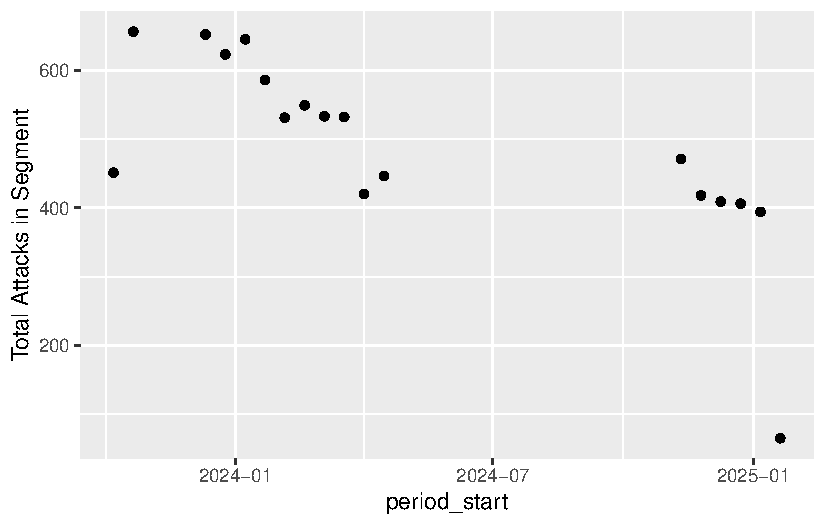
\includegraphics[keepaspectratio]{EDA_files/figure-pdf/unnamed-chunk-1-1.pdf}}

\begin{Shaded}
\begin{Highlighting}[]
\FunctionTok{ggplot}\NormalTok{(totaldata, }\FunctionTok{aes}\NormalTok{(}\AttributeTok{x =} \StringTok{\textasciigrave{}}\AttributeTok{Total Attacks in Segment}\StringTok{\textasciigrave{}}\NormalTok{, }\AttributeTok{y =}\NormalTok{ avg\_distance\_km)) }\SpecialCharTok{+}
  \FunctionTok{geom\_point}\NormalTok{()}
\end{Highlighting}
\end{Shaded}

\pandocbounded{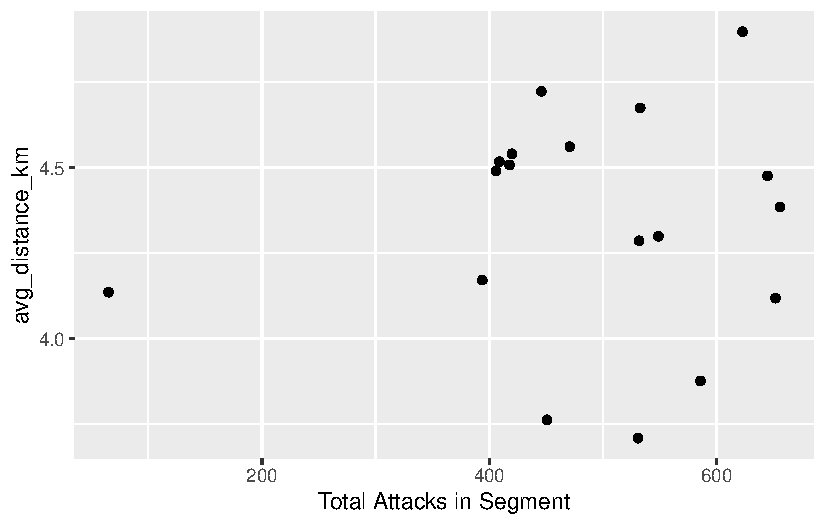
\includegraphics[keepaspectratio]{EDA_files/figure-pdf/unnamed-chunk-1-2.pdf}}

\begin{Shaded}
\begin{Highlighting}[]
\FunctionTok{ggplot}\NormalTok{(totaldata, }\FunctionTok{aes}\NormalTok{(}\AttributeTok{x =} \StringTok{\textasciigrave{}}\AttributeTok{Catchment Area (km²)}\StringTok{\textasciigrave{}}\NormalTok{, }\AttributeTok{y =} \StringTok{\textasciigrave{}}\AttributeTok{Percentage of Total Attacks}\StringTok{\textasciigrave{}}\NormalTok{)) }\SpecialCharTok{+}
  \FunctionTok{geom\_point}\NormalTok{()}
\end{Highlighting}
\end{Shaded}

\pandocbounded{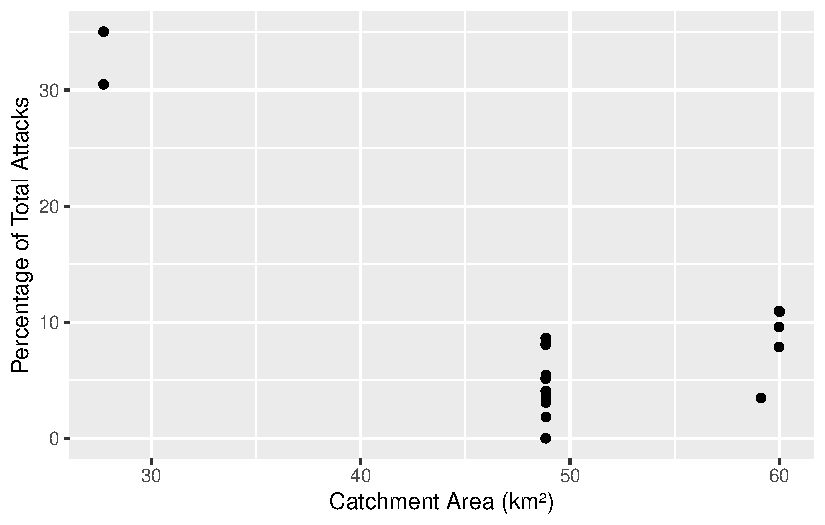
\includegraphics[keepaspectratio]{EDA_files/figure-pdf/unnamed-chunk-1-3.pdf}}

\begin{Shaded}
\begin{Highlighting}[]
\FunctionTok{ggplot}\NormalTok{(totaldata, }\FunctionTok{aes}\NormalTok{(}\AttributeTok{x =}\NormalTok{ avg\_distance\_km, }\AttributeTok{y =} \StringTok{\textasciigrave{}}\AttributeTok{Catchment Area (km²)}\StringTok{\textasciigrave{}}\NormalTok{)) }\SpecialCharTok{+}
  \FunctionTok{geom\_point}\NormalTok{()}
\end{Highlighting}
\end{Shaded}

\pandocbounded{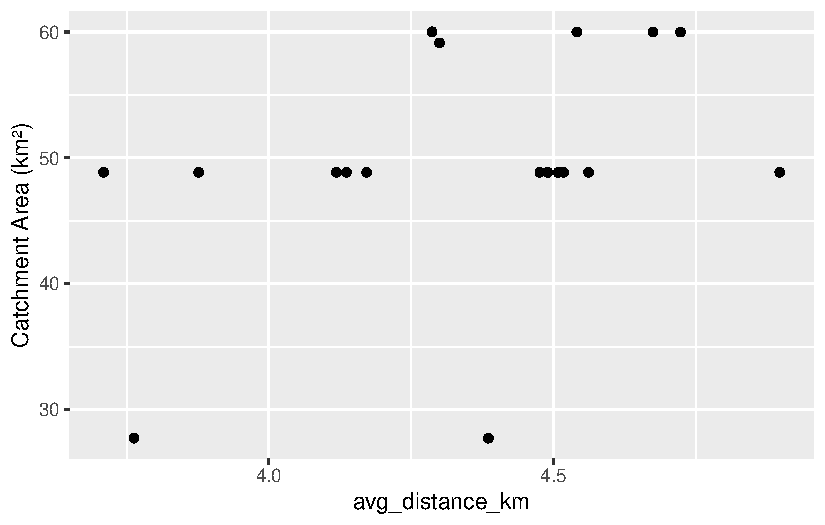
\includegraphics[keepaspectratio]{EDA_files/figure-pdf/unnamed-chunk-1-4.pdf}}

\begin{Shaded}
\begin{Highlighting}[]
\NormalTok{totaldata }\OtherTok{\textless{}{-}}\NormalTok{ totaldata }\SpecialCharTok{|\textgreater{}}
  \FunctionTok{mutate}\NormalTok{(}\AttributeTok{totinjuries =}\NormalTok{ Burn }\SpecialCharTok{+}\NormalTok{ CMF }\SpecialCharTok{+}\NormalTok{ Limb }\SpecialCharTok{+}\NormalTok{ NTD }\SpecialCharTok{+} \StringTok{\textasciigrave{}}\AttributeTok{Soft Tissue}\StringTok{\textasciigrave{}} \SpecialCharTok{+} \StringTok{\textasciigrave{}}\AttributeTok{Wound Care}\StringTok{\textasciigrave{}}\NormalTok{) }\SpecialCharTok{|\textgreater{}}
  \FunctionTok{mutate}\NormalTok{(}\AttributeTok{burnprop =}\NormalTok{ Burn }\SpecialCharTok{/}\NormalTok{ totinjuries) }\SpecialCharTok{|\textgreater{}}
  \FunctionTok{mutate}\NormalTok{(}\AttributeTok{cmfprop =}\NormalTok{ CMF }\SpecialCharTok{/}\NormalTok{ totinjuries) }\SpecialCharTok{|\textgreater{}}
  \FunctionTok{mutate}\NormalTok{(}\AttributeTok{limbprop =}\NormalTok{ Limb }\SpecialCharTok{/}\NormalTok{ totinjuries) }\SpecialCharTok{|\textgreater{}}
  \FunctionTok{mutate}\NormalTok{(}\AttributeTok{ntdprop =}\NormalTok{ NTD }\SpecialCharTok{/}\NormalTok{ totinjuries) }\SpecialCharTok{|\textgreater{}}
  \FunctionTok{mutate}\NormalTok{(}\AttributeTok{stprop =} \StringTok{\textasciigrave{}}\AttributeTok{Soft Tissue}\StringTok{\textasciigrave{}} \SpecialCharTok{/}\NormalTok{ totinjuries) }\SpecialCharTok{|\textgreater{}}
  \FunctionTok{mutate}\NormalTok{(}\AttributeTok{wcprop =} \StringTok{\textasciigrave{}}\AttributeTok{Wound Care}\StringTok{\textasciigrave{}} \SpecialCharTok{/}\NormalTok{ totinjuries)}

\NormalTok{totaldata }\OtherTok{\textless{}{-}}\NormalTok{ totaldata }\SpecialCharTok{|\textgreater{}}
  \FunctionTok{mutate}\NormalTok{(}\FunctionTok{across}\NormalTok{(}\FunctionTok{where}\NormalTok{(is.numeric), }\SpecialCharTok{\textasciitilde{}} \FunctionTok{replace}\NormalTok{(., }\FunctionTok{is.nan}\NormalTok{(.), }\DecValTok{0}\NormalTok{)))}
\end{Highlighting}
\end{Shaded}

\begin{Shaded}
\begin{Highlighting}[]
\CommentTok{\# Single robust chunk: uses exact "period\_start to period\_end" labels on x{-}axis.}
\CommentTok{\# All tidy functions are namespace{-}qualified to avoid masking issues (e.g. MASS::select).}
\CommentTok{\#}
\CommentTok{\# Requirements (install once if needed):}
\CommentTok{\# install.packages(c("readxl","dplyr","tidyr","ggplot2","lubridate","scales","stringr"))}

\CommentTok{\# {-}{-}{-} Libraries (not strictly necessary because we qualify most calls, but load for plotting defaults) {-}{-}{-}}
\CommentTok{\# It\textquotesingle{}s fine to load them but we won\textquotesingle{}t rely on unqualified function names.}
\FunctionTok{suppressMessages}\NormalTok{(\{}
  \FunctionTok{library}\NormalTok{(ggplot2)}
\NormalTok{\})}

\CommentTok{\# {-}{-}{-} Read the file (tries working dir then /mnt/data) {-}{-}{-}}
\NormalTok{xlsx\_candidates }\OtherTok{\textless{}{-}} \FunctionTok{c}\NormalTok{(}\StringTok{"aggregated\_dataset.xlsx"}\NormalTok{, }\StringTok{"/mnt/data/aggregated\_dataset.xlsx"}\NormalTok{)}
\NormalTok{dataset\_path }\OtherTok{\textless{}{-}} \ConstantTok{NULL}
\ControlFlowTok{for}\NormalTok{ (p }\ControlFlowTok{in}\NormalTok{ xlsx\_candidates) \{}
  \ControlFlowTok{if}\NormalTok{ (}\FunctionTok{file.exists}\NormalTok{(p)) \{ dataset\_path }\OtherTok{\textless{}{-}}\NormalTok{ p; }\ControlFlowTok{break}\NormalTok{ \}}
\NormalTok{\}}
\ControlFlowTok{if}\NormalTok{ (}\FunctionTok{is.null}\NormalTok{(dataset\_path)) }\FunctionTok{stop}\NormalTok{(}\StringTok{"Could not find aggregated\_dataset.xlsx. Place it in the working directory or /mnt/data/"}\NormalTok{)}

\NormalTok{df }\OtherTok{\textless{}{-}}\NormalTok{ readxl}\SpecialCharTok{::}\FunctionTok{read\_xlsx}\NormalTok{(dataset\_path)}

\CommentTok{\# {-}{-}{-} Normalize column names slightly (trim, collapse whitespace) {-}{-}{-}}
\NormalTok{orig\_names }\OtherTok{\textless{}{-}} \FunctionTok{names}\NormalTok{(df)}
\NormalTok{clean\_names }\OtherTok{\textless{}{-}}\NormalTok{ stringr}\SpecialCharTok{::}\FunctionTok{str\_trim}\NormalTok{(orig\_names)}
\NormalTok{clean\_names }\OtherTok{\textless{}{-}}\NormalTok{ stringr}\SpecialCharTok{::}\FunctionTok{str\_replace\_all}\NormalTok{(clean\_names, }\StringTok{"[}\SpecialCharTok{\textbackslash{}\textbackslash{}}\StringTok{s]+"}\NormalTok{, }\StringTok{" "}\NormalTok{)}
\FunctionTok{names}\NormalTok{(df) }\OtherTok{\textless{}{-}}\NormalTok{ clean\_names}
\NormalTok{lc\_names }\OtherTok{\textless{}{-}} \FunctionTok{tolower}\NormalTok{(clean\_names)}

\CommentTok{\# {-}{-}{-} Find biweekly start/end columns (fuzzy) {-}{-}{-}}
\NormalTok{possible\_start\_names }\OtherTok{\textless{}{-}} \FunctionTok{c}\NormalTok{(}\StringTok{"period\_start"}\NormalTok{, }\StringTok{"period start"}\NormalTok{, }\StringTok{"start\_date"}\NormalTok{, }\StringTok{"start"}\NormalTok{, }\StringTok{"periodstart"}\NormalTok{)}
\NormalTok{possible\_end\_names   }\OtherTok{\textless{}{-}} \FunctionTok{c}\NormalTok{(}\StringTok{"period\_end"}\NormalTok{, }\StringTok{"period end"}\NormalTok{, }\StringTok{"end\_date"}\NormalTok{, }\StringTok{"end"}\NormalTok{, }\StringTok{"periodend"}\NormalTok{)}

\NormalTok{find\_first\_match }\OtherTok{\textless{}{-}} \ControlFlowTok{function}\NormalTok{(cands, lc\_names, avail\_names) \{}
  \ControlFlowTok{for}\NormalTok{ (c }\ControlFlowTok{in}\NormalTok{ cands) \{}
\NormalTok{    i }\OtherTok{\textless{}{-}} \FunctionTok{which}\NormalTok{(lc\_names }\SpecialCharTok{==} \FunctionTok{tolower}\NormalTok{(c))}
    \ControlFlowTok{if}\NormalTok{ (}\FunctionTok{length}\NormalTok{(i) }\SpecialCharTok{\textgreater{}} \DecValTok{0}\NormalTok{) }\FunctionTok{return}\NormalTok{(avail\_names[i[}\DecValTok{1}\NormalTok{]])}
\NormalTok{  \}}
  \ControlFlowTok{for}\NormalTok{ (c }\ControlFlowTok{in}\NormalTok{ cands) \{}
\NormalTok{    i }\OtherTok{\textless{}{-}} \FunctionTok{which}\NormalTok{(stringr}\SpecialCharTok{::}\FunctionTok{str\_detect}\NormalTok{(lc\_names, stringr}\SpecialCharTok{::}\FunctionTok{str\_replace\_all}\NormalTok{(}\FunctionTok{tolower}\NormalTok{(c), }\StringTok{"[\^{}a{-}z0{-}9]+"}\NormalTok{, }\StringTok{".*"}\NormalTok{)))}
    \ControlFlowTok{if}\NormalTok{ (}\FunctionTok{length}\NormalTok{(i) }\SpecialCharTok{\textgreater{}} \DecValTok{0}\NormalTok{) }\FunctionTok{return}\NormalTok{(avail\_names[i[}\DecValTok{1}\NormalTok{]])}
\NormalTok{  \}}
  \FunctionTok{return}\NormalTok{(}\ConstantTok{NA\_character\_}\NormalTok{)}
\NormalTok{\}}
\NormalTok{start\_col }\OtherTok{\textless{}{-}} \FunctionTok{find\_first\_match}\NormalTok{(possible\_start\_names, lc\_names, }\FunctionTok{names}\NormalTok{(df))}
\NormalTok{end\_col   }\OtherTok{\textless{}{-}} \FunctionTok{find\_first\_match}\NormalTok{(possible\_end\_names, lc\_names, }\FunctionTok{names}\NormalTok{(df))}

\ControlFlowTok{if}\NormalTok{ (}\FunctionTok{is.na}\NormalTok{(start\_col) }\SpecialCharTok{|} \FunctionTok{is.na}\NormalTok{(end\_col)) }\FunctionTok{stop}\NormalTok{(}\StringTok{"Could not detect biweekly period start/end columns. Look for \textquotesingle{}period\_start\textquotesingle{}/\textquotesingle{}period\_end\textquotesingle{} or similar names."}\NormalTok{)}

\CommentTok{\# {-}{-}{-} Convert start/end to Date (handle POSIX, Date, or character with timezone) {-}{-}{-}}
\NormalTok{to\_date\_safe }\OtherTok{\textless{}{-}} \ControlFlowTok{function}\NormalTok{(x) \{}
  \ControlFlowTok{if}\NormalTok{ (}\FunctionTok{inherits}\NormalTok{(x, }\StringTok{"Date"}\NormalTok{)) }\FunctionTok{return}\NormalTok{(x)}
  \ControlFlowTok{if}\NormalTok{ (}\FunctionTok{inherits}\NormalTok{(x, }\StringTok{"POSIXt"}\NormalTok{)) }\FunctionTok{return}\NormalTok{(}\FunctionTok{as.Date}\NormalTok{(x))}
\NormalTok{  x\_chr }\OtherTok{\textless{}{-}} \FunctionTok{as.character}\NormalTok{(x)}
  \CommentTok{\# drop trailing " UTC" or timezone{-}like suffix}
\NormalTok{  x\_chr }\OtherTok{\textless{}{-}}\NormalTok{ stringr}\SpecialCharTok{::}\FunctionTok{str\_replace}\NormalTok{(x\_chr, }\StringTok{"}\SpecialCharTok{\textbackslash{}\textbackslash{}}\StringTok{s*UTC}\SpecialCharTok{\textbackslash{}\textbackslash{}}\StringTok{s*$"}\NormalTok{, }\StringTok{""}\NormalTok{)}
  \CommentTok{\# try ymd\_hms first, then ymd}
\NormalTok{  parsed\_hms }\OtherTok{\textless{}{-}} \FunctionTok{suppressWarnings}\NormalTok{(lubridate}\SpecialCharTok{::}\FunctionTok{ymd\_hms}\NormalTok{(x\_chr, }\AttributeTok{quiet =} \ConstantTok{TRUE}\NormalTok{))}
  \ControlFlowTok{if}\NormalTok{ (}\SpecialCharTok{!}\FunctionTok{all}\NormalTok{(}\FunctionTok{is.na}\NormalTok{(parsed\_hms))) }\FunctionTok{return}\NormalTok{(}\FunctionTok{as.Date}\NormalTok{(parsed\_hms))}
\NormalTok{  parsed }\OtherTok{\textless{}{-}} \FunctionTok{suppressWarnings}\NormalTok{(lubridate}\SpecialCharTok{::}\FunctionTok{ymd}\NormalTok{(x\_chr, }\AttributeTok{quiet =} \ConstantTok{TRUE}\NormalTok{))}
  \FunctionTok{as.Date}\NormalTok{(parsed)}
\NormalTok{\}}

\NormalTok{df[[start\_col]] }\OtherTok{\textless{}{-}} \FunctionTok{to\_date\_safe}\NormalTok{(df[[start\_col]])}
\NormalTok{df[[end\_col]]   }\OtherTok{\textless{}{-}} \FunctionTok{to\_date\_safe}\NormalTok{(df[[end\_col]])}

\CommentTok{\# {-}{-}{-} Create period label "YYYY{-}MM{-}DD to YYYY{-}MM{-}DD" and ordered factor by period start {-}{-}{-}}
\NormalTok{df }\OtherTok{\textless{}{-}}\NormalTok{ dplyr}\SpecialCharTok{::}\FunctionTok{arrange}\NormalTok{(df, .data[[start\_col]])}
\NormalTok{df }\OtherTok{\textless{}{-}}\NormalTok{ dplyr}\SpecialCharTok{::}\FunctionTok{mutate}\NormalTok{(df,}
                    \AttributeTok{period\_start\_date =} \FunctionTok{as.Date}\NormalTok{(.data[[start\_col]]),}
                    \AttributeTok{period\_end\_date   =} \FunctionTok{as.Date}\NormalTok{(.data[[end\_col]]),}
                    \AttributeTok{period\_label =} \FunctionTok{paste0}\NormalTok{(}\FunctionTok{format}\NormalTok{(period\_start\_date, }\StringTok{"\%Y{-}\%m{-}\%d"}\NormalTok{), }\StringTok{" to "}\NormalTok{, }\FunctionTok{format}\NormalTok{(period\_end\_date, }\StringTok{"\%Y{-}\%m{-}\%d"}\NormalTok{))}
\NormalTok{)}

\CommentTok{\# ordered factor so x{-}axis respects chronological order}
\NormalTok{df}\SpecialCharTok{$}\NormalTok{period\_label }\OtherTok{\textless{}{-}} \FunctionTok{factor}\NormalTok{(df}\SpecialCharTok{$}\NormalTok{period\_label, }\AttributeTok{levels =} \FunctionTok{unique}\NormalTok{(df}\SpecialCharTok{$}\NormalTok{period\_label))}

\CommentTok{\# {-}{-}{-} Define user variable groups (attempt fuzzy matching to actual columns) {-}{-}{-}}
\NormalTok{attack\_vars\_user }\OtherTok{\textless{}{-}} \FunctionTok{c}\NormalTok{(}\StringTok{"Air/drone strike"}\NormalTok{,}\StringTok{"Ground Attacks"}\NormalTok{,}\StringTok{"Shelling/artillery/missile attack"}\NormalTok{,}\StringTok{"Civil Unrest"}\NormalTok{,}\StringTok{"Other"}\NormalTok{)}
\NormalTok{injury\_vars\_user }\OtherTok{\textless{}{-}} \FunctionTok{c}\NormalTok{(}\StringTok{"Burn"}\NormalTok{,}\StringTok{"CMF"}\NormalTok{,}\StringTok{"Limb"}\NormalTok{,}\StringTok{"NTD"}\NormalTok{,}\StringTok{"Soft Tissue"}\NormalTok{,}\StringTok{"Wound Care"}\NormalTok{)}
\NormalTok{rest\_vars\_user   }\OtherTok{\textless{}{-}} \FunctionTok{c}\NormalTok{(}\StringTok{"avg\_distance\_km"}\NormalTok{,}\StringTok{"Catchment Area (km²)"}\NormalTok{,}\StringTok{"Attacks in Catchment"}\NormalTok{,}\StringTok{"Total Attacks in Segment"}\NormalTok{,}\StringTok{"Percentage of Total Attacks"}\NormalTok{,}\StringTok{"percent\_total\_area"}\NormalTok{)}

\NormalTok{fuzzy\_match }\OtherTok{\textless{}{-}} \ControlFlowTok{function}\NormalTok{(user\_vec, available\_names) \{}
\NormalTok{  avail\_lc }\OtherTok{\textless{}{-}} \FunctionTok{tolower}\NormalTok{(available\_names)}
\NormalTok{  res }\OtherTok{\textless{}{-}} \FunctionTok{character}\NormalTok{(}\FunctionTok{length}\NormalTok{(user\_vec))}
  \ControlFlowTok{for}\NormalTok{ (i }\ControlFlowTok{in} \FunctionTok{seq\_along}\NormalTok{(user\_vec)) \{}
\NormalTok{    u }\OtherTok{\textless{}{-}} \FunctionTok{tolower}\NormalTok{(user\_vec[i])}
\NormalTok{    exact\_idx }\OtherTok{\textless{}{-}} \FunctionTok{which}\NormalTok{(avail\_lc }\SpecialCharTok{==}\NormalTok{ u)}
    \ControlFlowTok{if}\NormalTok{ (}\FunctionTok{length}\NormalTok{(exact\_idx) }\SpecialCharTok{\textgreater{}} \DecValTok{0}\NormalTok{) \{ res[i] }\OtherTok{\textless{}{-}}\NormalTok{ available\_names[exact\_idx[}\DecValTok{1}\NormalTok{]]; }\ControlFlowTok{next}\NormalTok{ \}}
\NormalTok{    contains\_idx }\OtherTok{\textless{}{-}} \FunctionTok{which}\NormalTok{(stringr}\SpecialCharTok{::}\FunctionTok{str\_detect}\NormalTok{(avail\_lc, stringr}\SpecialCharTok{::}\FunctionTok{fixed}\NormalTok{(u)))}
    \ControlFlowTok{if}\NormalTok{ (}\FunctionTok{length}\NormalTok{(contains\_idx) }\SpecialCharTok{\textgreater{}} \DecValTok{0}\NormalTok{) \{ res[i] }\OtherTok{\textless{}{-}}\NormalTok{ available\_names[contains\_idx[}\DecValTok{1}\NormalTok{]]; }\ControlFlowTok{next}\NormalTok{ \}}
\NormalTok{    u\_norm }\OtherTok{\textless{}{-}}\NormalTok{ stringr}\SpecialCharTok{::}\FunctionTok{str\_replace\_all}\NormalTok{(u, }\StringTok{"[\^{}a{-}z0{-}9]+"}\NormalTok{, }\StringTok{""}\NormalTok{)}
\NormalTok{    norm\_idx }\OtherTok{\textless{}{-}} \FunctionTok{which}\NormalTok{(stringr}\SpecialCharTok{::}\FunctionTok{str\_replace\_all}\NormalTok{(avail\_lc, }\StringTok{"[\^{}a{-}z0{-}9]+"}\NormalTok{, }\StringTok{""}\NormalTok{) }\SpecialCharTok{==}\NormalTok{ u\_norm)}
    \ControlFlowTok{if}\NormalTok{ (}\FunctionTok{length}\NormalTok{(norm\_idx) }\SpecialCharTok{\textgreater{}} \DecValTok{0}\NormalTok{) \{ res[i] }\OtherTok{\textless{}{-}}\NormalTok{ available\_names[norm\_idx[}\DecValTok{1}\NormalTok{]]; }\ControlFlowTok{next}\NormalTok{ \}}
\NormalTok{    partial\_idx }\OtherTok{\textless{}{-}} \FunctionTok{which}\NormalTok{(stringr}\SpecialCharTok{::}\FunctionTok{str\_detect}\NormalTok{(avail\_lc, stringr}\SpecialCharTok{::}\FunctionTok{str\_replace\_all}\NormalTok{(u, }\StringTok{"[\^{}a{-}z0{-}9]+"}\NormalTok{, }\StringTok{".*"}\NormalTok{)))}
    \ControlFlowTok{if}\NormalTok{ (}\FunctionTok{length}\NormalTok{(partial\_idx) }\SpecialCharTok{\textgreater{}} \DecValTok{0}\NormalTok{) \{ res[i] }\OtherTok{\textless{}{-}}\NormalTok{ available\_names[partial\_idx[}\DecValTok{1}\NormalTok{]]; }\ControlFlowTok{next}\NormalTok{ \}}
\NormalTok{    res[i] }\OtherTok{\textless{}{-}} \ConstantTok{NA\_character\_}
\NormalTok{  \}}
\NormalTok{  res}
\NormalTok{\}}

\NormalTok{attack\_cols }\OtherTok{\textless{}{-}} \FunctionTok{fuzzy\_match}\NormalTok{(attack\_vars\_user, }\FunctionTok{names}\NormalTok{(df)); attack\_cols }\OtherTok{\textless{}{-}}\NormalTok{ attack\_cols[}\SpecialCharTok{!}\FunctionTok{is.na}\NormalTok{(attack\_cols)]}
\NormalTok{injury\_cols }\OtherTok{\textless{}{-}} \FunctionTok{fuzzy\_match}\NormalTok{(injury\_vars\_user, }\FunctionTok{names}\NormalTok{(df)); injury\_cols }\OtherTok{\textless{}{-}}\NormalTok{ injury\_cols[}\SpecialCharTok{!}\FunctionTok{is.na}\NormalTok{(injury\_cols)]}
\NormalTok{rest\_cols   }\OtherTok{\textless{}{-}} \FunctionTok{fuzzy\_match}\NormalTok{(rest\_vars\_user, }\FunctionTok{names}\NormalTok{(df));   rest\_cols   }\OtherTok{\textless{}{-}}\NormalTok{ rest\_cols[}\SpecialCharTok{!}\FunctionTok{is.na}\NormalTok{(rest\_cols)]}

\CommentTok{\# also add any percent/percentage columns to rest\_cols (useful)}
\NormalTok{pct\_cols }\OtherTok{\textless{}{-}} \FunctionTok{names}\NormalTok{(df)[stringr}\SpecialCharTok{::}\FunctionTok{str\_detect}\NormalTok{(}\FunctionTok{tolower}\NormalTok{(}\FunctionTok{names}\NormalTok{(df)), }\StringTok{"percent|percentage"}\NormalTok{)]}
\NormalTok{rest\_cols }\OtherTok{\textless{}{-}} \FunctionTok{unique}\NormalTok{(}\FunctionTok{c}\NormalTok{(rest\_cols, pct\_cols))}

\CommentTok{\# Diagnostic print}
\FunctionTok{cat}\NormalTok{(}\StringTok{"Using file:"}\NormalTok{, dataset\_path, }\StringTok{"}\SpecialCharTok{\textbackslash{}n}\StringTok{"}\NormalTok{)}
\end{Highlighting}
\end{Shaded}

\begin{verbatim}
Using file: aggregated_dataset.xlsx 
\end{verbatim}

\begin{Shaded}
\begin{Highlighting}[]
\FunctionTok{cat}\NormalTok{(}\StringTok{"Period start col:"}\NormalTok{, start\_col, }\StringTok{"end col:"}\NormalTok{, end\_col, }\StringTok{"}\SpecialCharTok{\textbackslash{}n}\StringTok{"}\NormalTok{)}
\end{Highlighting}
\end{Shaded}

\begin{verbatim}
Period start col: period_start end col: period_end 
\end{verbatim}

\begin{Shaded}
\begin{Highlighting}[]
\FunctionTok{cat}\NormalTok{(}\StringTok{"Periods (first/last):"}\NormalTok{, }\FunctionTok{as.character}\NormalTok{(}\FunctionTok{first}\NormalTok{(df}\SpecialCharTok{$}\NormalTok{period\_label)), }\StringTok{" ... "}\NormalTok{, }\FunctionTok{as.character}\NormalTok{(}\FunctionTok{last}\NormalTok{(df}\SpecialCharTok{$}\NormalTok{period\_label)), }\StringTok{"}\SpecialCharTok{\textbackslash{}n}\StringTok{"}\NormalTok{)}
\end{Highlighting}
\end{Shaded}

\begin{verbatim}
Periods (first/last): 2023-10-07 to 2023-10-20  ...  2025-01-20 to 2025-02-02 
\end{verbatim}

\begin{Shaded}
\begin{Highlighting}[]
\FunctionTok{cat}\NormalTok{(}\StringTok{"Attack columns found:"}\NormalTok{, }\ControlFlowTok{if}\NormalTok{(}\FunctionTok{length}\NormalTok{(attack\_cols)}\SpecialCharTok{\textgreater{}}\DecValTok{0}\NormalTok{) }\FunctionTok{paste}\NormalTok{(attack\_cols, }\AttributeTok{collapse=}\StringTok{", "}\NormalTok{) }\ControlFlowTok{else} \StringTok{"NONE"}\NormalTok{, }\StringTok{"}\SpecialCharTok{\textbackslash{}n}\StringTok{"}\NormalTok{)}
\end{Highlighting}
\end{Shaded}

\begin{verbatim}
Attack columns found: Air/drone strike, Ground Attacks, Shelling/artillery/missile attack, Civil Unrest, Other 
\end{verbatim}

\begin{Shaded}
\begin{Highlighting}[]
\FunctionTok{cat}\NormalTok{(}\StringTok{"Injury columns found:"}\NormalTok{, }\ControlFlowTok{if}\NormalTok{(}\FunctionTok{length}\NormalTok{(injury\_cols)}\SpecialCharTok{\textgreater{}}\DecValTok{0}\NormalTok{) }\FunctionTok{paste}\NormalTok{(injury\_cols, }\AttributeTok{collapse=}\StringTok{", "}\NormalTok{) }\ControlFlowTok{else} \StringTok{"NONE"}\NormalTok{, }\StringTok{"}\SpecialCharTok{\textbackslash{}n}\StringTok{"}\NormalTok{)}
\end{Highlighting}
\end{Shaded}

\begin{verbatim}
Injury columns found: Burn, CMF, Limb, NTD, Soft Tissue, Wound Care 
\end{verbatim}

\begin{Shaded}
\begin{Highlighting}[]
\FunctionTok{cat}\NormalTok{(}\StringTok{"Rest columns found:"}\NormalTok{, }\ControlFlowTok{if}\NormalTok{(}\FunctionTok{length}\NormalTok{(rest\_cols)}\SpecialCharTok{\textgreater{}}\DecValTok{0}\NormalTok{) }\FunctionTok{paste}\NormalTok{(rest\_cols, }\AttributeTok{collapse=}\StringTok{", "}\NormalTok{) }\ControlFlowTok{else} \StringTok{"NONE"}\NormalTok{, }\StringTok{"}\SpecialCharTok{\textbackslash{}n\textbackslash{}n}\StringTok{"}\NormalTok{)}
\end{Highlighting}
\end{Shaded}

\begin{verbatim}
Rest columns found: avg_distance_km, Catchment Area (km²), Attacks in Catchment, Total Attacks in Segment, Percentage of Total Attacks, percent_total_area 
\end{verbatim}

\begin{Shaded}
\begin{Highlighting}[]
\CommentTok{\# {-}{-}{-} helper numeric coercion {-}{-}{-}}
\NormalTok{to\_num }\OtherTok{\textless{}{-}} \ControlFlowTok{function}\NormalTok{(x) }\FunctionTok{suppressWarnings}\NormalTok{(}\FunctionTok{as.numeric}\NormalTok{(x))}

\CommentTok{\# {-}{-}{-} 1) Attack types plot (x = period\_label categorical) {-}{-}{-}}
\ControlFlowTok{if}\NormalTok{ (}\FunctionTok{length}\NormalTok{(attack\_cols) }\SpecialCharTok{\textgreater{}} \DecValTok{0}\NormalTok{) \{}
\NormalTok{  attacks\_long }\OtherTok{\textless{}{-}}\NormalTok{ df }\SpecialCharTok{\%\textgreater{}\%}
\NormalTok{    dplyr}\SpecialCharTok{::}\FunctionTok{select}\NormalTok{(period\_label, dplyr}\SpecialCharTok{::}\FunctionTok{all\_of}\NormalTok{(attack\_cols)) }\SpecialCharTok{\%\textgreater{}\%}
\NormalTok{    tidyr}\SpecialCharTok{::}\FunctionTok{pivot\_longer}\NormalTok{(}\AttributeTok{cols =} \SpecialCharTok{{-}}\NormalTok{period\_label, }\AttributeTok{names\_to =} \StringTok{"attack\_type"}\NormalTok{, }\AttributeTok{values\_to =} \StringTok{"value"}\NormalTok{) }\SpecialCharTok{\%\textgreater{}\%}
\NormalTok{    dplyr}\SpecialCharTok{::}\FunctionTok{mutate}\NormalTok{(}\AttributeTok{value =} \FunctionTok{to\_num}\NormalTok{(value),}
                  \AttributeTok{attack\_type =} \FunctionTok{factor}\NormalTok{(attack\_type, }\AttributeTok{levels =} \FunctionTok{unique}\NormalTok{(attack\_type)))}
  
\NormalTok{  p\_attacks }\OtherTok{\textless{}{-}}\NormalTok{ ggplot2}\SpecialCharTok{::}\FunctionTok{ggplot}\NormalTok{(attacks\_long, ggplot2}\SpecialCharTok{::}\FunctionTok{aes}\NormalTok{(}\AttributeTok{x=}\NormalTok{period\_label, }\AttributeTok{y=}\NormalTok{value, }\AttributeTok{group=}\NormalTok{attack\_type, }\AttributeTok{color=}\NormalTok{attack\_type)) }\SpecialCharTok{+}
\NormalTok{    ggplot2}\SpecialCharTok{::}\FunctionTok{geom\_line}\NormalTok{(}\AttributeTok{size=}\DecValTok{1}\NormalTok{) }\SpecialCharTok{+}
\NormalTok{    ggplot2}\SpecialCharTok{::}\FunctionTok{geom\_point}\NormalTok{(}\AttributeTok{size=}\DecValTok{2}\NormalTok{) }\SpecialCharTok{+}
\NormalTok{    ggplot2}\SpecialCharTok{::}\FunctionTok{labs}\NormalTok{(}\AttributeTok{title=}\StringTok{"Attack types over biweekly periods"}\NormalTok{, }\AttributeTok{x=}\StringTok{"Biweekly period"}\NormalTok{, }\AttributeTok{y=}\StringTok{"Count"}\NormalTok{, }\AttributeTok{color=}\StringTok{"Attack Type"}\NormalTok{) }\SpecialCharTok{+}
\NormalTok{    ggplot2}\SpecialCharTok{::}\FunctionTok{theme\_minimal}\NormalTok{() }\SpecialCharTok{+}
\NormalTok{    ggplot2}\SpecialCharTok{::}\FunctionTok{theme}\NormalTok{(}\AttributeTok{axis.text.x =}\NormalTok{ ggplot2}\SpecialCharTok{::}\FunctionTok{element\_text}\NormalTok{(}\AttributeTok{angle =} \DecValTok{45}\NormalTok{, }\AttributeTok{hjust =} \DecValTok{1}\NormalTok{), }\AttributeTok{plot.title =}\NormalTok{ ggplot2}\SpecialCharTok{::}\FunctionTok{element\_text}\NormalTok{(}\AttributeTok{hjust=}\FloatTok{0.5}\NormalTok{))}
  \FunctionTok{print}\NormalTok{(p\_attacks)}
\NormalTok{\} }\ControlFlowTok{else}\NormalTok{ \{}
  \FunctionTok{plot.new}\NormalTok{(); }\FunctionTok{text}\NormalTok{(}\FloatTok{0.5}\NormalTok{,}\FloatTok{0.5}\NormalTok{,}\StringTok{"No attack columns found to plot"}\NormalTok{)}
\NormalTok{\}}
\end{Highlighting}
\end{Shaded}

\begin{verbatim}
Warning: Using `size` aesthetic for lines was deprecated in ggplot2 3.4.0.
i Please use `linewidth` instead.
\end{verbatim}

\pandocbounded{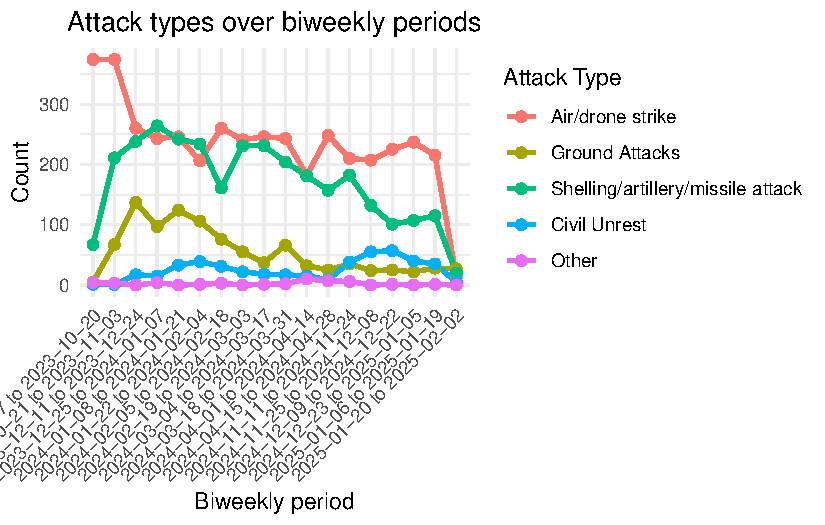
\includegraphics[keepaspectratio]{EDA_files/figure-pdf/initial-chat-plots-1.pdf}}

\begin{Shaded}
\begin{Highlighting}[]
\CommentTok{\# {-}{-}{-} 2) Injury types plot {-}{-}{-}}
\ControlFlowTok{if}\NormalTok{ (}\FunctionTok{length}\NormalTok{(injury\_cols) }\SpecialCharTok{\textgreater{}} \DecValTok{0}\NormalTok{) \{}
\NormalTok{  inj\_long }\OtherTok{\textless{}{-}}\NormalTok{ df }\SpecialCharTok{\%\textgreater{}\%}
\NormalTok{    dplyr}\SpecialCharTok{::}\FunctionTok{select}\NormalTok{(period\_label, dplyr}\SpecialCharTok{::}\FunctionTok{all\_of}\NormalTok{(injury\_cols)) }\SpecialCharTok{\%\textgreater{}\%}
\NormalTok{    tidyr}\SpecialCharTok{::}\FunctionTok{pivot\_longer}\NormalTok{(}\AttributeTok{cols =} \SpecialCharTok{{-}}\NormalTok{period\_label, }\AttributeTok{names\_to =} \StringTok{"injury\_type"}\NormalTok{, }\AttributeTok{values\_to =} \StringTok{"value"}\NormalTok{) }\SpecialCharTok{\%\textgreater{}\%}
\NormalTok{    dplyr}\SpecialCharTok{::}\FunctionTok{mutate}\NormalTok{(}\AttributeTok{value =} \FunctionTok{to\_num}\NormalTok{(value),}
                  \AttributeTok{injury\_type =} \FunctionTok{factor}\NormalTok{(injury\_type, }\AttributeTok{levels =} \FunctionTok{unique}\NormalTok{(injury\_type)))}
  
\NormalTok{  p\_injuries }\OtherTok{\textless{}{-}}\NormalTok{ ggplot2}\SpecialCharTok{::}\FunctionTok{ggplot}\NormalTok{(inj\_long, ggplot2}\SpecialCharTok{::}\FunctionTok{aes}\NormalTok{(}\AttributeTok{x=}\NormalTok{period\_label, }\AttributeTok{y=}\NormalTok{value, }\AttributeTok{group=}\NormalTok{injury\_type, }\AttributeTok{color=}\NormalTok{injury\_type)) }\SpecialCharTok{+}
\NormalTok{    ggplot2}\SpecialCharTok{::}\FunctionTok{geom\_line}\NormalTok{(}\AttributeTok{size=}\DecValTok{1}\NormalTok{) }\SpecialCharTok{+}
\NormalTok{    ggplot2}\SpecialCharTok{::}\FunctionTok{geom\_point}\NormalTok{(}\AttributeTok{size=}\DecValTok{2}\NormalTok{) }\SpecialCharTok{+}
\NormalTok{    ggplot2}\SpecialCharTok{::}\FunctionTok{labs}\NormalTok{(}\AttributeTok{title=}\StringTok{"Injury types over biweekly periods"}\NormalTok{, }\AttributeTok{x=}\StringTok{"Biweekly period"}\NormalTok{, }\AttributeTok{y=}\StringTok{"Count"}\NormalTok{, }\AttributeTok{color=}\StringTok{"Injury Type"}\NormalTok{) }\SpecialCharTok{+}
\NormalTok{    ggplot2}\SpecialCharTok{::}\FunctionTok{theme\_minimal}\NormalTok{() }\SpecialCharTok{+}
\NormalTok{    ggplot2}\SpecialCharTok{::}\FunctionTok{theme}\NormalTok{(}\AttributeTok{axis.text.x =}\NormalTok{ ggplot2}\SpecialCharTok{::}\FunctionTok{element\_text}\NormalTok{(}\AttributeTok{angle =} \DecValTok{45}\NormalTok{, }\AttributeTok{hjust =} \DecValTok{1}\NormalTok{), }\AttributeTok{plot.title =}\NormalTok{ ggplot2}\SpecialCharTok{::}\FunctionTok{element\_text}\NormalTok{(}\AttributeTok{hjust=}\FloatTok{0.5}\NormalTok{))}
  \FunctionTok{print}\NormalTok{(p\_injuries)}
\NormalTok{\} }\ControlFlowTok{else}\NormalTok{ \{}
  \FunctionTok{plot.new}\NormalTok{(); }\FunctionTok{text}\NormalTok{(}\FloatTok{0.5}\NormalTok{,}\FloatTok{0.5}\NormalTok{,}\StringTok{"No injury columns found to plot"}\NormalTok{)}
\NormalTok{\}}
\end{Highlighting}
\end{Shaded}

\pandocbounded{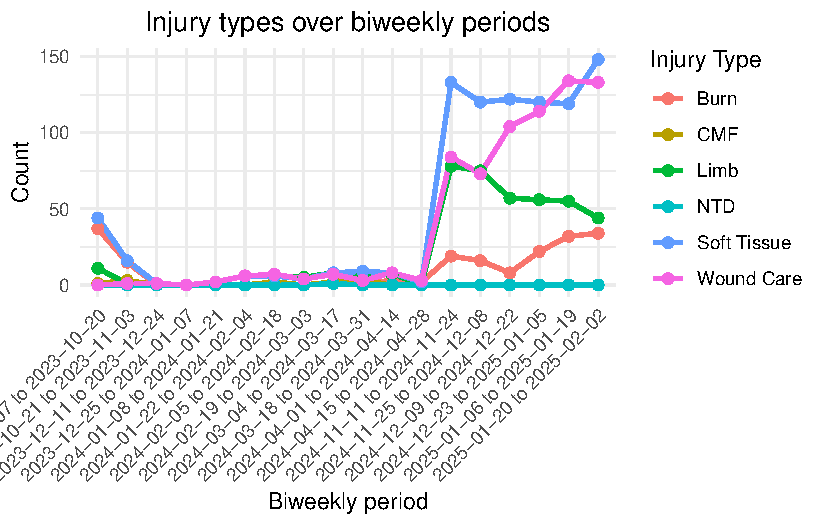
\includegraphics[keepaspectratio]{EDA_files/figure-pdf/initial-chat-plots-2.pdf}}

\begin{Shaded}
\begin{Highlighting}[]
\CommentTok{\# {-}{-}{-} 3) Rest variables combined (min{-}max scaled) with categorical x {-}{-}{-}}
\ControlFlowTok{if}\NormalTok{ (}\FunctionTok{length}\NormalTok{(rest\_cols) }\SpecialCharTok{\textgreater{}} \DecValTok{0}\NormalTok{) \{}
\NormalTok{  rest\_long }\OtherTok{\textless{}{-}}\NormalTok{ df }\SpecialCharTok{\%\textgreater{}\%}
\NormalTok{    dplyr}\SpecialCharTok{::}\FunctionTok{select}\NormalTok{(period\_label, dplyr}\SpecialCharTok{::}\FunctionTok{all\_of}\NormalTok{(rest\_cols)) }\SpecialCharTok{\%\textgreater{}\%}
\NormalTok{    tidyr}\SpecialCharTok{::}\FunctionTok{pivot\_longer}\NormalTok{(}\AttributeTok{cols =} \SpecialCharTok{{-}}\NormalTok{period\_label, }\AttributeTok{names\_to =} \StringTok{"var"}\NormalTok{, }\AttributeTok{values\_to =} \StringTok{"value"}\NormalTok{) }\SpecialCharTok{\%\textgreater{}\%}
\NormalTok{    dplyr}\SpecialCharTok{::}\FunctionTok{mutate}\NormalTok{(}\AttributeTok{value\_num =} \FunctionTok{to\_num}\NormalTok{(value)) }\SpecialCharTok{\%\textgreater{}\%}
\NormalTok{    dplyr}\SpecialCharTok{::}\FunctionTok{group\_by}\NormalTok{(var) }\SpecialCharTok{\%\textgreater{}\%}
\NormalTok{    dplyr}\SpecialCharTok{::}\FunctionTok{mutate}\NormalTok{(}\AttributeTok{min\_v =} \FunctionTok{min}\NormalTok{(value\_num, }\AttributeTok{na.rm=}\ConstantTok{TRUE}\NormalTok{),}
                  \AttributeTok{max\_v =} \FunctionTok{max}\NormalTok{(value\_num, }\AttributeTok{na.rm=}\ConstantTok{TRUE}\NormalTok{),}
                  \AttributeTok{scaled =} \FunctionTok{ifelse}\NormalTok{(}\FunctionTok{is.finite}\NormalTok{(min\_v) }\SpecialCharTok{\&} \FunctionTok{is.finite}\NormalTok{(max\_v) }\SpecialCharTok{\&}\NormalTok{ (max\_v }\SpecialCharTok{{-}}\NormalTok{ min\_v) }\SpecialCharTok{\textgreater{}} \DecValTok{0}\NormalTok{,}
\NormalTok{                                  (value\_num }\SpecialCharTok{{-}}\NormalTok{ min\_v) }\SpecialCharTok{/}\NormalTok{ (max\_v }\SpecialCharTok{{-}}\NormalTok{ min\_v),}
                                  \ConstantTok{NA\_real\_}\NormalTok{)) }\SpecialCharTok{\%\textgreater{}\%}
\NormalTok{    dplyr}\SpecialCharTok{::}\FunctionTok{ungroup}\NormalTok{()}
  
\NormalTok{  p\_rest\_scaled }\OtherTok{\textless{}{-}}\NormalTok{ ggplot2}\SpecialCharTok{::}\FunctionTok{ggplot}\NormalTok{(rest\_long, ggplot2}\SpecialCharTok{::}\FunctionTok{aes}\NormalTok{(}\AttributeTok{x=}\NormalTok{period\_label, }\AttributeTok{y=}\NormalTok{scaled, }\AttributeTok{group=}\NormalTok{var, }\AttributeTok{color=}\NormalTok{var)) }\SpecialCharTok{+}
\NormalTok{    ggplot2}\SpecialCharTok{::}\FunctionTok{geom\_line}\NormalTok{(}\AttributeTok{size=}\DecValTok{1}\NormalTok{) }\SpecialCharTok{+}
\NormalTok{    ggplot2}\SpecialCharTok{::}\FunctionTok{geom\_point}\NormalTok{(}\AttributeTok{size=}\FloatTok{1.6}\NormalTok{) }\SpecialCharTok{+}
\NormalTok{    ggplot2}\SpecialCharTok{::}\FunctionTok{labs}\NormalTok{(}\AttributeTok{title=}\StringTok{"Other variables (min{-}max scaled) across biweekly periods"}\NormalTok{, }\AttributeTok{x=}\StringTok{"Biweekly period"}\NormalTok{, }\AttributeTok{y=}\StringTok{"Scaled (0{-}1)"}\NormalTok{, }\AttributeTok{color=}\StringTok{"Variable"}\NormalTok{) }\SpecialCharTok{+}
\NormalTok{    ggplot2}\SpecialCharTok{::}\FunctionTok{theme\_minimal}\NormalTok{() }\SpecialCharTok{+}
\NormalTok{    ggplot2}\SpecialCharTok{::}\FunctionTok{theme}\NormalTok{(}\AttributeTok{axis.text.x =}\NormalTok{ ggplot2}\SpecialCharTok{::}\FunctionTok{element\_text}\NormalTok{(}\AttributeTok{angle =} \DecValTok{45}\NormalTok{, }\AttributeTok{hjust =} \DecValTok{1}\NormalTok{), }\AttributeTok{plot.title =}\NormalTok{ ggplot2}\SpecialCharTok{::}\FunctionTok{element\_text}\NormalTok{(}\AttributeTok{hjust=}\FloatTok{0.5}\NormalTok{))}
  \FunctionTok{print}\NormalTok{(p\_rest\_scaled)}
  
  \CommentTok{\# small multiples: raw values}
\NormalTok{  rest\_long\_raw }\OtherTok{\textless{}{-}}\NormalTok{ rest\_long }\SpecialCharTok{\%\textgreater{}\%}\NormalTok{ dplyr}\SpecialCharTok{::}\FunctionTok{mutate}\NormalTok{(}\AttributeTok{value\_num =} \FunctionTok{as.numeric}\NormalTok{(value\_num))}
\NormalTok{  p\_rest\_facets }\OtherTok{\textless{}{-}}\NormalTok{ ggplot2}\SpecialCharTok{::}\FunctionTok{ggplot}\NormalTok{(rest\_long\_raw, ggplot2}\SpecialCharTok{::}\FunctionTok{aes}\NormalTok{(}\AttributeTok{x=}\NormalTok{period\_label, }\AttributeTok{y=}\NormalTok{value\_num, }\AttributeTok{group=}\DecValTok{1}\NormalTok{)) }\SpecialCharTok{+}
\NormalTok{    ggplot2}\SpecialCharTok{::}\FunctionTok{geom\_line}\NormalTok{() }\SpecialCharTok{+}\NormalTok{ ggplot2}\SpecialCharTok{::}\FunctionTok{geom\_point}\NormalTok{(}\AttributeTok{size=}\DecValTok{1}\NormalTok{) }\SpecialCharTok{+}
\NormalTok{    ggplot2}\SpecialCharTok{::}\FunctionTok{facet\_wrap}\NormalTok{(}\SpecialCharTok{\textasciitilde{}}\NormalTok{var, }\AttributeTok{scales=}\StringTok{"free\_y"}\NormalTok{, }\AttributeTok{ncol=}\DecValTok{2}\NormalTok{) }\SpecialCharTok{+}
\NormalTok{    ggplot2}\SpecialCharTok{::}\FunctionTok{labs}\NormalTok{(}\AttributeTok{title=}\StringTok{"Other variables (raw values) — one panel per variable"}\NormalTok{, }\AttributeTok{x=}\StringTok{"Biweekly period"}\NormalTok{, }\AttributeTok{y=}\StringTok{"Value"}\NormalTok{) }\SpecialCharTok{+}
\NormalTok{    ggplot2}\SpecialCharTok{::}\FunctionTok{theme\_minimal}\NormalTok{() }\SpecialCharTok{+}
\NormalTok{    ggplot2}\SpecialCharTok{::}\FunctionTok{theme}\NormalTok{(}\AttributeTok{axis.text.x =}\NormalTok{ ggplot2}\SpecialCharTok{::}\FunctionTok{element\_text}\NormalTok{(}\AttributeTok{angle =} \DecValTok{45}\NormalTok{, }\AttributeTok{hjust =} \DecValTok{1}\NormalTok{), }\AttributeTok{plot.title =}\NormalTok{ ggplot2}\SpecialCharTok{::}\FunctionTok{element\_text}\NormalTok{(}\AttributeTok{hjust=}\FloatTok{0.5}\NormalTok{))}
  \FunctionTok{print}\NormalTok{(p\_rest\_facets)}
  
\NormalTok{\} }\ControlFlowTok{else}\NormalTok{ \{}
  \FunctionTok{plot.new}\NormalTok{(); }\FunctionTok{text}\NormalTok{(}\FloatTok{0.5}\NormalTok{,}\FloatTok{0.5}\NormalTok{,}\StringTok{"No \textquotesingle{}rest\textquotesingle{} variables found to plot"}\NormalTok{)}
\NormalTok{\}}
\end{Highlighting}
\end{Shaded}

\pandocbounded{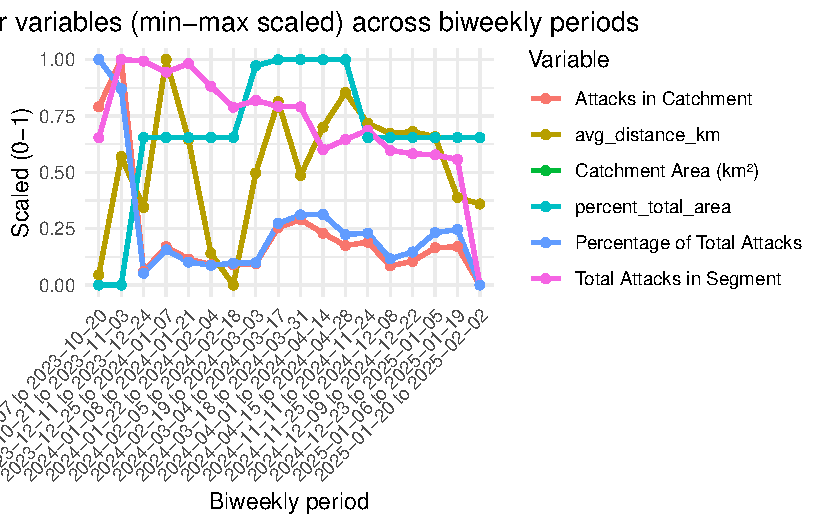
\includegraphics[keepaspectratio]{EDA_files/figure-pdf/initial-chat-plots-3.pdf}}

\pandocbounded{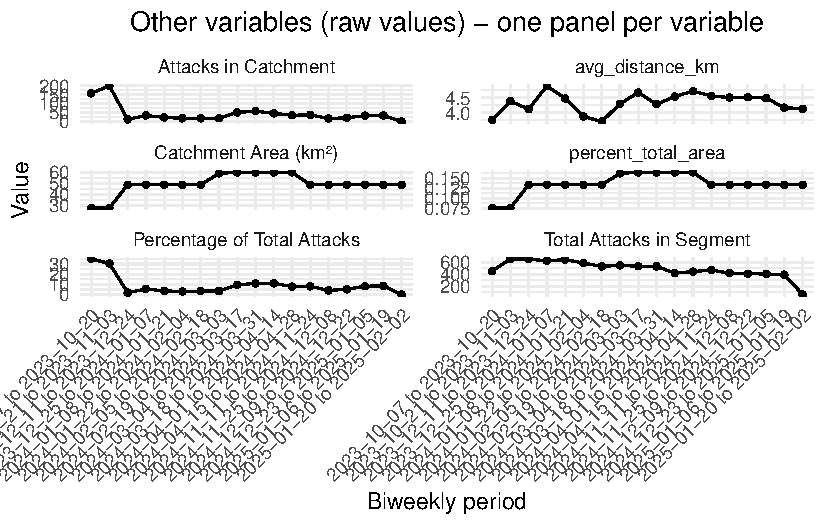
\includegraphics[keepaspectratio]{EDA_files/figure-pdf/initial-chat-plots-4.pdf}}

\begin{Shaded}
\begin{Highlighting}[]
\CommentTok{\# {-}{-}{-} 4) Big plot: all variables together (min{-}max scaled) across categorical x{-}axis {-}{-}{-}}
\NormalTok{all\_plot\_cols }\OtherTok{\textless{}{-}} \FunctionTok{unique}\NormalTok{(}\FunctionTok{c}\NormalTok{(attack\_cols, injury\_cols, rest\_cols))}
\NormalTok{all\_plot\_cols }\OtherTok{\textless{}{-}}\NormalTok{ all\_plot\_cols[}\SpecialCharTok{!}\FunctionTok{is.na}\NormalTok{(all\_plot\_cols)]}
\ControlFlowTok{if}\NormalTok{ (}\FunctionTok{length}\NormalTok{(all\_plot\_cols) }\SpecialCharTok{\textgreater{}} \DecValTok{0}\NormalTok{) \{}
\NormalTok{  all\_long }\OtherTok{\textless{}{-}}\NormalTok{ df }\SpecialCharTok{\%\textgreater{}\%}
\NormalTok{    dplyr}\SpecialCharTok{::}\FunctionTok{select}\NormalTok{(period\_label, dplyr}\SpecialCharTok{::}\FunctionTok{all\_of}\NormalTok{(all\_plot\_cols)) }\SpecialCharTok{\%\textgreater{}\%}
\NormalTok{    tidyr}\SpecialCharTok{::}\FunctionTok{pivot\_longer}\NormalTok{(}\AttributeTok{cols =} \SpecialCharTok{{-}}\NormalTok{period\_label, }\AttributeTok{names\_to =} \StringTok{"var"}\NormalTok{, }\AttributeTok{values\_to =} \StringTok{"value"}\NormalTok{) }\SpecialCharTok{\%\textgreater{}\%}
\NormalTok{    dplyr}\SpecialCharTok{::}\FunctionTok{mutate}\NormalTok{(}\AttributeTok{value\_num =} \FunctionTok{to\_num}\NormalTok{(value)) }\SpecialCharTok{\%\textgreater{}\%}
\NormalTok{    dplyr}\SpecialCharTok{::}\FunctionTok{group\_by}\NormalTok{(var) }\SpecialCharTok{\%\textgreater{}\%}
\NormalTok{    dplyr}\SpecialCharTok{::}\FunctionTok{mutate}\NormalTok{(}\AttributeTok{min\_v =} \FunctionTok{min}\NormalTok{(value\_num, }\AttributeTok{na.rm=}\ConstantTok{TRUE}\NormalTok{),}
                  \AttributeTok{max\_v =} \FunctionTok{max}\NormalTok{(value\_num, }\AttributeTok{na.rm=}\ConstantTok{TRUE}\NormalTok{),}
                  \AttributeTok{scaled =} \FunctionTok{ifelse}\NormalTok{(}\FunctionTok{is.finite}\NormalTok{(min\_v) }\SpecialCharTok{\&} \FunctionTok{is.finite}\NormalTok{(max\_v) }\SpecialCharTok{\&}\NormalTok{ (max\_v }\SpecialCharTok{{-}}\NormalTok{ min\_v) }\SpecialCharTok{\textgreater{}} \DecValTok{0}\NormalTok{,}
\NormalTok{                                  (value\_num }\SpecialCharTok{{-}}\NormalTok{ min\_v) }\SpecialCharTok{/}\NormalTok{ (max\_v }\SpecialCharTok{{-}}\NormalTok{ min\_v),}
                                  \ConstantTok{NA\_real\_}\NormalTok{)) }\SpecialCharTok{\%\textgreater{}\%}
\NormalTok{    dplyr}\SpecialCharTok{::}\FunctionTok{ungroup}\NormalTok{()}
  
\NormalTok{  p\_all }\OtherTok{\textless{}{-}}\NormalTok{ ggplot2}\SpecialCharTok{::}\FunctionTok{ggplot}\NormalTok{(all\_long, ggplot2}\SpecialCharTok{::}\FunctionTok{aes}\NormalTok{(}\AttributeTok{x=}\NormalTok{period\_label, }\AttributeTok{y=}\NormalTok{scaled, }\AttributeTok{group=}\NormalTok{var, }\AttributeTok{color=}\NormalTok{var)) }\SpecialCharTok{+}
\NormalTok{    ggplot2}\SpecialCharTok{::}\FunctionTok{geom\_line}\NormalTok{(}\AttributeTok{size=}\FloatTok{0.9}\NormalTok{) }\SpecialCharTok{+}
\NormalTok{    ggplot2}\SpecialCharTok{::}\FunctionTok{geom\_point}\NormalTok{(}\AttributeTok{size=}\FloatTok{1.2}\NormalTok{) }\SpecialCharTok{+}
\NormalTok{    ggplot2}\SpecialCharTok{::}\FunctionTok{labs}\NormalTok{(}\AttributeTok{title=}\StringTok{"All variables together (min{-}max scaled per variable) across biweekly periods"}\NormalTok{, }\AttributeTok{x=}\StringTok{"Biweekly period"}\NormalTok{, }\AttributeTok{y=}\StringTok{"Scaled (0{-}1)"}\NormalTok{, }\AttributeTok{color=}\StringTok{"Variable"}\NormalTok{) }\SpecialCharTok{+}
\NormalTok{    ggplot2}\SpecialCharTok{::}\FunctionTok{theme\_minimal}\NormalTok{() }\SpecialCharTok{+}
\NormalTok{    ggplot2}\SpecialCharTok{::}\FunctionTok{theme}\NormalTok{(}\AttributeTok{axis.text.x =}\NormalTok{ ggplot2}\SpecialCharTok{::}\FunctionTok{element\_text}\NormalTok{(}\AttributeTok{angle =} \DecValTok{45}\NormalTok{, }\AttributeTok{hjust =} \DecValTok{1}\NormalTok{), }\AttributeTok{plot.title =}\NormalTok{ ggplot2}\SpecialCharTok{::}\FunctionTok{element\_text}\NormalTok{(}\AttributeTok{hjust=}\FloatTok{0.5}\NormalTok{))}
  \FunctionTok{print}\NormalTok{(p\_all)}
\NormalTok{\} }\ControlFlowTok{else}\NormalTok{ \{}
  \FunctionTok{plot.new}\NormalTok{(); }\FunctionTok{text}\NormalTok{(}\FloatTok{0.5}\NormalTok{,}\FloatTok{0.5}\NormalTok{,}\StringTok{"No variables found to include in the \textquotesingle{}all variables\textquotesingle{} plot"}\NormalTok{)}
\NormalTok{\}}
\end{Highlighting}
\end{Shaded}

\pandocbounded{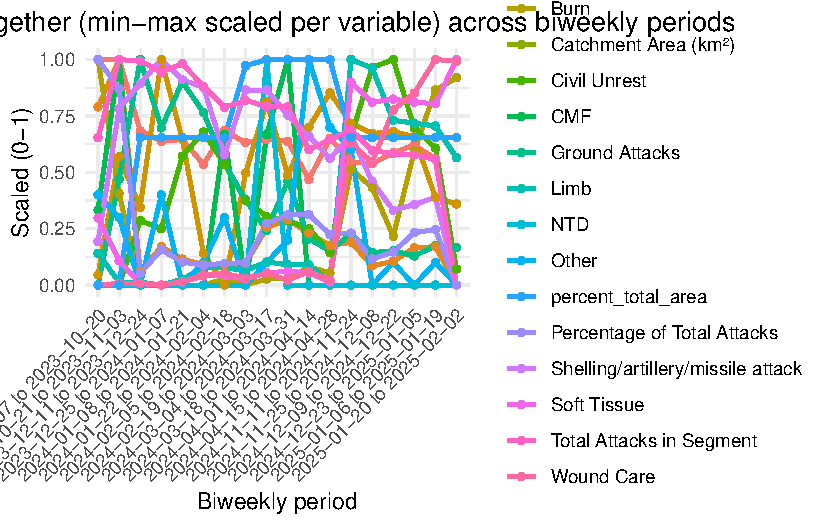
\includegraphics[keepaspectratio]{EDA_files/figure-pdf/initial-chat-plots-5.pdf}}

\begin{Shaded}
\begin{Highlighting}[]
\CommentTok{\# {-}{-}{-} End of chunk {-}{-}{-}}
\CommentTok{\# Tips:}
\CommentTok{\# {-} To reduce x{-}axis label crowding, show only every N{-}th label:}
\CommentTok{\#     + Add: + scale\_x\_discrete(breaks = levels(df$period\_label)[seq(1, nlevels(df$period\_label), by = 2)])}
\CommentTok{\# {-} To change scaling to z{-}scores:}
\CommentTok{\#     replace the \textquotesingle{}scaled\textquotesingle{} calculation with:}
\CommentTok{\#       scaled = (value\_num {-} mean(value\_num, na.rm=TRUE)) / sd(value\_num, na.rm=TRUE)}
\CommentTok{\# {-} If you want lines to *not* connect across calendar gaps (when using date x rather than categorical),}
\CommentTok{\#   I can add logic to create break groups. With the categorical period\_label approach (used above),}
\CommentTok{\#   spacing is even and lines connect only adjacent periods.}
\end{Highlighting}
\end{Shaded}

\begin{Shaded}
\begin{Highlighting}[]
\CommentTok{\#totaldata |\textgreater{}}
  \CommentTok{\#filter(\textasciigrave{}Hospital\textasciigrave{} == "Al Shifa Medical Hospital") |\textgreater{}}
  
  
\CommentTok{\# Namespace{-}safe chunk: group injuries by hospital (Al Shifa, European, Nasser) and plot distributions.}
\CommentTok{\# Requires: readxl, dplyr, tidyr, ggplot2, stringr}
\CommentTok{\# Install if needed: install.packages(c("readxl","dplyr","tidyr","ggplot2","stringr"))}

\CommentTok{\# Load a plotting library (we\textquotesingle{}ll fully qualify other functions)}
\FunctionTok{suppressMessages}\NormalTok{(\{ }\FunctionTok{library}\NormalTok{(ggplot2) \})}

\CommentTok{\# {-}{-}{-} Read file {-}{-}{-}}
\NormalTok{xlsx\_candidates }\OtherTok{\textless{}{-}} \FunctionTok{c}\NormalTok{(}\StringTok{"aggregated\_dataset.xlsx"}\NormalTok{, }\StringTok{"/mnt/data/aggregated\_dataset.xlsx"}\NormalTok{)}
\NormalTok{dataset\_path }\OtherTok{\textless{}{-}} \ConstantTok{NULL}
\ControlFlowTok{for}\NormalTok{ (p }\ControlFlowTok{in}\NormalTok{ xlsx\_candidates) }\ControlFlowTok{if}\NormalTok{ (}\FunctionTok{file.exists}\NormalTok{(p)) \{ dataset\_path }\OtherTok{\textless{}{-}}\NormalTok{ p; }\ControlFlowTok{break}\NormalTok{ \}}
\ControlFlowTok{if}\NormalTok{ (}\FunctionTok{is.null}\NormalTok{(dataset\_path)) }\FunctionTok{stop}\NormalTok{(}\StringTok{"Could not find aggregated\_dataset.xlsx. Place it in the working directory or /mnt/data/"}\NormalTok{)}

\NormalTok{df }\OtherTok{\textless{}{-}}\NormalTok{ readxl}\SpecialCharTok{::}\FunctionTok{read\_xlsx}\NormalTok{(dataset\_path)}

\CommentTok{\# {-}{-}{-} Normalize column names {-}{-}{-}}
\FunctionTok{names}\NormalTok{(df) }\OtherTok{\textless{}{-}}\NormalTok{ stringr}\SpecialCharTok{::}\FunctionTok{str\_trim}\NormalTok{(}\FunctionTok{names}\NormalTok{(df))}
\FunctionTok{names}\NormalTok{(df) }\OtherTok{\textless{}{-}}\NormalTok{ stringr}\SpecialCharTok{::}\FunctionTok{str\_replace\_all}\NormalTok{(}\FunctionTok{names}\NormalTok{(df), }\StringTok{"[}\SpecialCharTok{\textbackslash{}\textbackslash{}}\StringTok{s]+"}\NormalTok{, }\StringTok{" "}\NormalTok{)  }\CommentTok{\# collapse multi{-}spaces}
\NormalTok{lc\_names }\OtherTok{\textless{}{-}} \FunctionTok{tolower}\NormalTok{(}\FunctionTok{names}\NormalTok{(df))}

\CommentTok{\# {-}{-}{-} 1) Find a hospital column (try common names) {-}{-}{-}}
\NormalTok{hospital\_candidates }\OtherTok{\textless{}{-}} \FunctionTok{c}\NormalTok{(}\StringTok{"hospital"}\NormalTok{, }\StringTok{"hospital\_name"}\NormalTok{, }\StringTok{"facility"}\NormalTok{, }\StringTok{"facility\_name"}\NormalTok{, }\StringTok{"site"}\NormalTok{, }\StringTok{"site\_name"}\NormalTok{, }\StringTok{"facility name"}\NormalTok{, }\StringTok{"hospital name"}\NormalTok{)}
\NormalTok{hospital\_col }\OtherTok{\textless{}{-}} \ConstantTok{NA\_character\_}
\ControlFlowTok{for}\NormalTok{ (cand }\ControlFlowTok{in}\NormalTok{ hospital\_candidates) \{}
\NormalTok{  i }\OtherTok{\textless{}{-}} \FunctionTok{which}\NormalTok{(lc\_names }\SpecialCharTok{==} \FunctionTok{tolower}\NormalTok{(cand))}
  \ControlFlowTok{if}\NormalTok{ (}\FunctionTok{length}\NormalTok{(i)}\SpecialCharTok{\textgreater{}}\DecValTok{0}\NormalTok{) \{ hospital\_col }\OtherTok{\textless{}{-}} \FunctionTok{names}\NormalTok{(df)[i[}\DecValTok{1}\NormalTok{]]; }\ControlFlowTok{break}\NormalTok{ \}}
\NormalTok{\}}
\CommentTok{\# fuzzy contains if exact not found}
\ControlFlowTok{if}\NormalTok{ (}\FunctionTok{is.na}\NormalTok{(hospital\_col)) \{}
  \ControlFlowTok{for}\NormalTok{ (cand }\ControlFlowTok{in}\NormalTok{ hospital\_candidates) \{}
\NormalTok{    i }\OtherTok{\textless{}{-}} \FunctionTok{which}\NormalTok{(stringr}\SpecialCharTok{::}\FunctionTok{str\_detect}\NormalTok{(lc\_names, stringr}\SpecialCharTok{::}\FunctionTok{str\_replace\_all}\NormalTok{(}\FunctionTok{tolower}\NormalTok{(cand), }\StringTok{"[\^{}a{-}z0{-}9]+"}\NormalTok{, }\StringTok{".*"}\NormalTok{)))}
    \ControlFlowTok{if}\NormalTok{ (}\FunctionTok{length}\NormalTok{(i)}\SpecialCharTok{\textgreater{}}\DecValTok{0}\NormalTok{) \{ hospital\_col }\OtherTok{\textless{}{-}} \FunctionTok{names}\NormalTok{(df)[i[}\DecValTok{1}\NormalTok{]]; }\ControlFlowTok{break}\NormalTok{ \}}
\NormalTok{  \}}
\NormalTok{\}}

\ControlFlowTok{if}\NormalTok{ (}\FunctionTok{is.na}\NormalTok{(hospital\_col)) \{}
  \FunctionTok{warning}\NormalTok{(}\StringTok{"No hospital/facility column detected. I will attempt to proceed by looking for hospital names in all character columns."}\NormalTok{)}
\NormalTok{\}}

\CommentTok{\# {-}{-}{-} 2) Define the injury type names we expect (user{-}provided list) {-}{-}{-}}
\NormalTok{injury\_vars\_user }\OtherTok{\textless{}{-}} \FunctionTok{c}\NormalTok{(}\StringTok{"Burn"}\NormalTok{,}\StringTok{"CMF"}\NormalTok{,}\StringTok{"Limb"}\NormalTok{,}\StringTok{"NTD"}\NormalTok{,}\StringTok{"Soft Tissue"}\NormalTok{,}\StringTok{"Wound Care"}\NormalTok{)}

\CommentTok{\# fuzzy matcher to find actual injury columns in df}
\NormalTok{fuzzy\_match\_cols }\OtherTok{\textless{}{-}} \ControlFlowTok{function}\NormalTok{(user\_vec, available\_names) \{}
\NormalTok{  avail\_lc }\OtherTok{\textless{}{-}} \FunctionTok{tolower}\NormalTok{(available\_names)}
  \FunctionTok{sapply}\NormalTok{(user\_vec, }\ControlFlowTok{function}\NormalTok{(u)\{}
\NormalTok{    u\_lc }\OtherTok{\textless{}{-}} \FunctionTok{tolower}\NormalTok{(u)}
    \CommentTok{\# exact}
\NormalTok{    idx }\OtherTok{\textless{}{-}} \FunctionTok{which}\NormalTok{(avail\_lc }\SpecialCharTok{==}\NormalTok{ u\_lc); }\ControlFlowTok{if}\NormalTok{ (}\FunctionTok{length}\NormalTok{(idx)}\SpecialCharTok{\textgreater{}}\DecValTok{0}\NormalTok{) }\FunctionTok{return}\NormalTok{(available\_names[idx[}\DecValTok{1}\NormalTok{]])}
    \CommentTok{\# contains}
\NormalTok{    idx }\OtherTok{\textless{}{-}} \FunctionTok{which}\NormalTok{(stringr}\SpecialCharTok{::}\FunctionTok{str\_detect}\NormalTok{(avail\_lc, stringr}\SpecialCharTok{::}\FunctionTok{fixed}\NormalTok{(u\_lc))); }\ControlFlowTok{if}\NormalTok{ (}\FunctionTok{length}\NormalTok{(idx)}\SpecialCharTok{\textgreater{}}\DecValTok{0}\NormalTok{) }\FunctionTok{return}\NormalTok{(available\_names[idx[}\DecValTok{1}\NormalTok{]])}
    \CommentTok{\# normalized (remove non{-}alphanum)}
\NormalTok{    u\_norm }\OtherTok{\textless{}{-}}\NormalTok{ stringr}\SpecialCharTok{::}\FunctionTok{str\_replace\_all}\NormalTok{(u\_lc, }\StringTok{"[\^{}a{-}z0{-}9]+"}\NormalTok{, }\StringTok{""}\NormalTok{)}
\NormalTok{    idx }\OtherTok{\textless{}{-}} \FunctionTok{which}\NormalTok{(stringr}\SpecialCharTok{::}\FunctionTok{str\_replace\_all}\NormalTok{(avail\_lc, }\StringTok{"[\^{}a{-}z0{-}9]+"}\NormalTok{, }\StringTok{""}\NormalTok{) }\SpecialCharTok{==}\NormalTok{ u\_norm); }\ControlFlowTok{if}\NormalTok{ (}\FunctionTok{length}\NormalTok{(idx)}\SpecialCharTok{\textgreater{}}\DecValTok{0}\NormalTok{) }\FunctionTok{return}\NormalTok{(available\_names[idx[}\DecValTok{1}\NormalTok{]])}
    \CommentTok{\# partial word{-}match}
\NormalTok{    idx }\OtherTok{\textless{}{-}} \FunctionTok{which}\NormalTok{(stringr}\SpecialCharTok{::}\FunctionTok{str\_detect}\NormalTok{(avail\_lc, stringr}\SpecialCharTok{::}\FunctionTok{str\_replace\_all}\NormalTok{(u\_lc, }\StringTok{"[\^{}a{-}z0{-}9]+"}\NormalTok{, }\StringTok{".*"}\NormalTok{))); }\ControlFlowTok{if}\NormalTok{ (}\FunctionTok{length}\NormalTok{(idx)}\SpecialCharTok{\textgreater{}}\DecValTok{0}\NormalTok{) }\FunctionTok{return}\NormalTok{(available\_names[idx[}\DecValTok{1}\NormalTok{]])}
    \ConstantTok{NA\_character\_}
\NormalTok{  \}, }\AttributeTok{USE.NAMES =} \ConstantTok{FALSE}\NormalTok{)}
\NormalTok{\}}

\NormalTok{injury\_cols }\OtherTok{\textless{}{-}} \FunctionTok{fuzzy\_match\_cols}\NormalTok{(injury\_vars\_user, }\FunctionTok{names}\NormalTok{(df))}
\NormalTok{injury\_map }\OtherTok{\textless{}{-}} \FunctionTok{data.frame}\NormalTok{(}\AttributeTok{requested =}\NormalTok{ injury\_vars\_user, }\AttributeTok{matched =}\NormalTok{ injury\_cols, }\AttributeTok{stringsAsFactors =} \ConstantTok{FALSE}\NormalTok{)}
\CommentTok{\# drop NA matches}
\NormalTok{injury\_cols\_clean }\OtherTok{\textless{}{-}} \FunctionTok{unique}\NormalTok{(}\FunctionTok{na.omit}\NormalTok{(injury\_cols))}

\ControlFlowTok{if}\NormalTok{ (}\FunctionTok{length}\NormalTok{(injury\_cols\_clean) }\SpecialCharTok{==} \DecValTok{0}\NormalTok{) }\FunctionTok{stop}\NormalTok{(}\StringTok{"No injury columns (Burn/CMF/Limb/NTD/Soft Tissue/Wound Care) were found. Check column names."}\NormalTok{)}

\CommentTok{\# Show mapping for user\textquotesingle{}s info}
\FunctionTok{cat}\NormalTok{(}\StringTok{"Injury columns matched:}\SpecialCharTok{\textbackslash{}n}\StringTok{"}\NormalTok{)}
\end{Highlighting}
\end{Shaded}

\begin{verbatim}
Injury columns matched:
\end{verbatim}

\begin{Shaded}
\begin{Highlighting}[]
\FunctionTok{print}\NormalTok{(injury\_map)}
\end{Highlighting}
\end{Shaded}

\begin{verbatim}
    requested     matched
1        Burn        Burn
2         CMF         CMF
3        Limb        Limb
4         NTD         NTD
5 Soft Tissue Soft Tissue
6  Wound Care  Wound Care
\end{verbatim}

\begin{Shaded}
\begin{Highlighting}[]
\CommentTok{\# {-}{-}{-} 3) Identify rows for each hospital (case{-}insensitive contains) {-}{-}{-}}
\CommentTok{\# We\textquotesingle{}ll look for these three hospital name fragments:}
\NormalTok{hospital\_targets }\OtherTok{\textless{}{-}} \FunctionTok{c}\NormalTok{(}\StringTok{"al shifa"}\NormalTok{, }\StringTok{"european"}\NormalTok{, }\StringTok{"nasser"}\NormalTok{)}

\CommentTok{\# Helper to find values in hospital\_col OR across all character columns if hospital\_col missing}
\NormalTok{find\_rows\_for\_hospital }\OtherTok{\textless{}{-}} \ControlFlowTok{function}\NormalTok{(df, hosp\_pattern) \{}
  \ControlFlowTok{if}\NormalTok{ (}\SpecialCharTok{!}\FunctionTok{is.na}\NormalTok{(hospital\_col)) \{}
\NormalTok{    vals }\OtherTok{\textless{}{-}} \FunctionTok{as.character}\NormalTok{(df[[hospital\_col]])}
\NormalTok{    sel }\OtherTok{\textless{}{-}}\NormalTok{ stringr}\SpecialCharTok{::}\FunctionTok{str\_detect}\NormalTok{(}\FunctionTok{tolower}\NormalTok{(vals), stringr}\SpecialCharTok{::}\FunctionTok{fixed}\NormalTok{(hosp\_pattern))}
    \FunctionTok{return}\NormalTok{(}\FunctionTok{which}\NormalTok{(sel))}
\NormalTok{  \} }\ControlFlowTok{else}\NormalTok{ \{}
    \CommentTok{\# search across all character columns}
\NormalTok{    char\_cols }\OtherTok{\textless{}{-}} \FunctionTok{names}\NormalTok{(df)[}\FunctionTok{sapply}\NormalTok{(df, }\ControlFlowTok{function}\NormalTok{(x) }\FunctionTok{is.character}\NormalTok{(x) }\SpecialCharTok{||} \FunctionTok{is.factor}\NormalTok{(x))]}
    \ControlFlowTok{if}\NormalTok{ (}\FunctionTok{length}\NormalTok{(char\_cols)}\SpecialCharTok{==}\DecValTok{0}\NormalTok{) }\FunctionTok{return}\NormalTok{(}\FunctionTok{integer}\NormalTok{(}\DecValTok{0}\NormalTok{))}
\NormalTok{    sel\_any }\OtherTok{\textless{}{-}} \FunctionTok{rep}\NormalTok{(}\ConstantTok{FALSE}\NormalTok{, }\FunctionTok{nrow}\NormalTok{(df))}
    \ControlFlowTok{for}\NormalTok{ (c }\ControlFlowTok{in}\NormalTok{ char\_cols) \{}
\NormalTok{      sel\_any }\OtherTok{\textless{}{-}}\NormalTok{ sel\_any }\SpecialCharTok{|}\NormalTok{ stringr}\SpecialCharTok{::}\FunctionTok{str\_detect}\NormalTok{(}\FunctionTok{tolower}\NormalTok{(}\FunctionTok{as.character}\NormalTok{(df[[c]])), stringr}\SpecialCharTok{::}\FunctionTok{fixed}\NormalTok{(hosp\_pattern))}
\NormalTok{    \}}
    \FunctionTok{return}\NormalTok{(}\FunctionTok{which}\NormalTok{(sel\_any))}
\NormalTok{  \}}
\NormalTok{\}}

\CommentTok{\# Collect the indices for each hospital}
\NormalTok{hospital\_indices }\OtherTok{\textless{}{-}} \FunctionTok{lapply}\NormalTok{(hospital\_targets, }\ControlFlowTok{function}\NormalTok{(pat) }\FunctionTok{find\_rows\_for\_hospital}\NormalTok{(df, pat))}
\FunctionTok{names}\NormalTok{(hospital\_indices) }\OtherTok{\textless{}{-}}\NormalTok{ hospital\_targets}

\CommentTok{\# Diagnostics: any not found?}
\ControlFlowTok{for}\NormalTok{ (i }\ControlFlowTok{in} \FunctionTok{seq\_along}\NormalTok{(hospital\_targets)) \{}
\NormalTok{  target }\OtherTok{\textless{}{-}}\NormalTok{ hospital\_targets[i]}
\NormalTok{  idx }\OtherTok{\textless{}{-}}\NormalTok{ hospital\_indices[[i]]}
  \ControlFlowTok{if}\NormalTok{ (}\FunctionTok{length}\NormalTok{(idx)}\SpecialCharTok{==}\DecValTok{0}\NormalTok{) }\FunctionTok{message}\NormalTok{(}\FunctionTok{sprintf}\NormalTok{(}\StringTok{"Warning: No rows found for hospital matching \textquotesingle{}\%s\textquotesingle{}."}\NormalTok{, target))}
  \ControlFlowTok{else} \FunctionTok{message}\NormalTok{(}\FunctionTok{sprintf}\NormalTok{(}\StringTok{"Found \%d rows for hospital matching \textquotesingle{}\%s\textquotesingle{}."}\NormalTok{, }\FunctionTok{length}\NormalTok{(idx), target))}
\NormalTok{\}}
\end{Highlighting}
\end{Shaded}

\begin{verbatim}
Found 2 rows for hospital matching 'al shifa'.
\end{verbatim}

\begin{verbatim}
Found 10 rows for hospital matching 'european'.
\end{verbatim}

\begin{verbatim}
Found 6 rows for hospital matching 'nasser'.
\end{verbatim}

\begin{Shaded}
\begin{Highlighting}[]
\CommentTok{\# {-}{-}{-} 4) For each hospital, sum the injury counts across rows and prepare a tidy table {-}{-}{-}}
\NormalTok{to\_num }\OtherTok{\textless{}{-}} \ControlFlowTok{function}\NormalTok{(x) }\FunctionTok{suppressWarnings}\NormalTok{(}\FunctionTok{as.numeric}\NormalTok{(x))}

\NormalTok{hospital\_summaries }\OtherTok{\textless{}{-}} \FunctionTok{list}\NormalTok{()}
\ControlFlowTok{for}\NormalTok{ (i }\ControlFlowTok{in} \FunctionTok{seq\_along}\NormalTok{(hospital\_targets)) \{}
\NormalTok{  target }\OtherTok{\textless{}{-}}\NormalTok{ hospital\_targets[i]}
\NormalTok{  idx }\OtherTok{\textless{}{-}}\NormalTok{ hospital\_indices[[i]]}
  \ControlFlowTok{if}\NormalTok{ (}\FunctionTok{length}\NormalTok{(idx)}\SpecialCharTok{==}\DecValTok{0}\NormalTok{) \{}
\NormalTok{    hospital\_summaries[[target]] }\OtherTok{\textless{}{-}} \ConstantTok{NULL}
    \ControlFlowTok{next}
\NormalTok{  \}}
  \CommentTok{\# subset rows and select the matched injury columns}
\NormalTok{  sub }\OtherTok{\textless{}{-}}\NormalTok{ df[idx, , drop }\OtherTok{=} \ConstantTok{FALSE}\NormalTok{]}
  \CommentTok{\# ensure columns exist in sub}
\NormalTok{  present\_inj\_cols }\OtherTok{\textless{}{-}} \FunctionTok{intersect}\NormalTok{(injury\_cols\_clean, }\FunctionTok{names}\NormalTok{(sub))}
  \ControlFlowTok{if}\NormalTok{ (}\FunctionTok{length}\NormalTok{(present\_inj\_cols)}\SpecialCharTok{==}\DecValTok{0}\NormalTok{) \{}
\NormalTok{    hospital\_summaries[[target]] }\OtherTok{\textless{}{-}} \ConstantTok{NULL}
    \ControlFlowTok{next}
\NormalTok{  \}}
  \CommentTok{\# coerce to numeric \& sum}
\NormalTok{  sums }\OtherTok{\textless{}{-}} \FunctionTok{sapply}\NormalTok{(present\_inj\_cols, }\ControlFlowTok{function}\NormalTok{(col) }\FunctionTok{sum}\NormalTok{(}\FunctionTok{to\_num}\NormalTok{(sub[[col]]), }\AttributeTok{na.rm =} \ConstantTok{TRUE}\NormalTok{))}
\NormalTok{  sums\_df }\OtherTok{\textless{}{-}} \FunctionTok{data.frame}\NormalTok{(}\AttributeTok{hospital =}\NormalTok{ target,}
                        \AttributeTok{injury\_type =} \FunctionTok{names}\NormalTok{(sums),}
                        \AttributeTok{count =} \FunctionTok{as.numeric}\NormalTok{(sums),}
                        \AttributeTok{stringsAsFactors =} \ConstantTok{FALSE}\NormalTok{)}
  \CommentTok{\# Make injury\_type labels prettier (use original requested name when matched)}
  \CommentTok{\# Map back to requested if possible:}
\NormalTok{  sums\_df}\SpecialCharTok{$}\NormalTok{injury\_label }\OtherTok{\textless{}{-}} \FunctionTok{sapply}\NormalTok{(sums\_df}\SpecialCharTok{$}\NormalTok{injury\_type, }\ControlFlowTok{function}\NormalTok{(matched) \{}
    \CommentTok{\# find first requested whose matched equals this matched}
\NormalTok{    req\_idx }\OtherTok{\textless{}{-}} \FunctionTok{which}\NormalTok{(injury\_map}\SpecialCharTok{$}\NormalTok{matched }\SpecialCharTok{==}\NormalTok{ matched)}
    \ControlFlowTok{if}\NormalTok{ (}\FunctionTok{length}\NormalTok{(req\_idx)}\SpecialCharTok{\textgreater{}}\DecValTok{0}\NormalTok{) injury\_map}\SpecialCharTok{$}\NormalTok{requested[req\_idx[}\DecValTok{1}\NormalTok{]] }\ControlFlowTok{else}\NormalTok{ matched}
\NormalTok{  \})}
\NormalTok{  hospital\_summaries[[target]] }\OtherTok{\textless{}{-}}\NormalTok{ sums\_df}
\NormalTok{\}}

\CommentTok{\# Combine summaries into one data.frame}
\NormalTok{summary\_combined }\OtherTok{\textless{}{-}} \FunctionTok{do.call}\NormalTok{(rbind, hospital\_summaries)}
\ControlFlowTok{if}\NormalTok{ (}\FunctionTok{is.null}\NormalTok{(summary\_combined) }\SpecialCharTok{||} \FunctionTok{nrow}\NormalTok{(summary\_combined)}\SpecialCharTok{==}\DecValTok{0}\NormalTok{) }\FunctionTok{stop}\NormalTok{(}\StringTok{"No hospital injury summaries could be computed. Check that hospital names and injury columns exist in the data."}\NormalTok{)}

\CommentTok{\# Reorder injury\_label factor to keep consistent ordering}
\NormalTok{summary\_combined}\SpecialCharTok{$}\NormalTok{injury\_label }\OtherTok{\textless{}{-}} \FunctionTok{factor}\NormalTok{(summary\_combined}\SpecialCharTok{$}\NormalTok{injury\_label, }\AttributeTok{levels =} \FunctionTok{unique}\NormalTok{(summary\_combined}\SpecialCharTok{$}\NormalTok{injury\_label))}

\CommentTok{\# {-}{-}{-} 5) Plot: one bar plot per hospital (printed sequentially) {-}{-}{-}}
\NormalTok{unique\_hospitals\_found }\OtherTok{\textless{}{-}} \FunctionTok{unique}\NormalTok{(summary\_combined}\SpecialCharTok{$}\NormalTok{hospital)}

\ControlFlowTok{for}\NormalTok{ (h }\ControlFlowTok{in}\NormalTok{ unique\_hospitals\_found) \{}
\NormalTok{  d\_h }\OtherTok{\textless{}{-}}\NormalTok{ summary\_combined[summary\_combined}\SpecialCharTok{$}\NormalTok{hospital }\SpecialCharTok{==}\NormalTok{ h, , drop }\OtherTok{=} \ConstantTok{FALSE}\NormalTok{]}
  \CommentTok{\# use requested hospital display name (title{-}case)}
\NormalTok{  display\_name }\OtherTok{\textless{}{-}}\NormalTok{ stringr}\SpecialCharTok{::}\FunctionTok{str\_to\_title}\NormalTok{(h)}
\NormalTok{  p }\OtherTok{\textless{}{-}}\NormalTok{ ggplot2}\SpecialCharTok{::}\FunctionTok{ggplot}\NormalTok{(d\_h, ggplot2}\SpecialCharTok{::}\FunctionTok{aes}\NormalTok{(}\AttributeTok{x =}\NormalTok{ injury\_label, }\AttributeTok{y =}\NormalTok{ count, }\AttributeTok{fill =}\NormalTok{ injury\_label)) }\SpecialCharTok{+}
\NormalTok{    ggplot2}\SpecialCharTok{::}\FunctionTok{geom\_col}\NormalTok{(}\AttributeTok{show.legend =} \ConstantTok{FALSE}\NormalTok{) }\SpecialCharTok{+}
\NormalTok{    ggplot2}\SpecialCharTok{::}\FunctionTok{geom\_text}\NormalTok{(ggplot2}\SpecialCharTok{::}\FunctionTok{aes}\NormalTok{(}\AttributeTok{label =}\NormalTok{ count), }\AttributeTok{vjust =} \SpecialCharTok{{-}}\FloatTok{0.25}\NormalTok{, }\AttributeTok{size =} \DecValTok{3}\NormalTok{) }\SpecialCharTok{+}
\NormalTok{    ggplot2}\SpecialCharTok{::}\FunctionTok{labs}\NormalTok{(}\AttributeTok{title =} \FunctionTok{paste0}\NormalTok{(display\_name, }\StringTok{" — Injury distribution (sum)"}\NormalTok{),}
                  \AttributeTok{x =} \StringTok{"Injury type"}\NormalTok{, }\AttributeTok{y =} \StringTok{"Total count (sum)"}\NormalTok{) }\SpecialCharTok{+}
\NormalTok{    ggplot2}\SpecialCharTok{::}\FunctionTok{theme\_minimal}\NormalTok{() }\SpecialCharTok{+}
\NormalTok{    ggplot2}\SpecialCharTok{::}\FunctionTok{theme}\NormalTok{(}\AttributeTok{axis.text.x =}\NormalTok{ ggplot2}\SpecialCharTok{::}\FunctionTok{element\_text}\NormalTok{(}\AttributeTok{angle =} \DecValTok{45}\NormalTok{, }\AttributeTok{hjust =} \DecValTok{1}\NormalTok{),}
                   \AttributeTok{plot.title =}\NormalTok{ ggplot2}\SpecialCharTok{::}\FunctionTok{element\_text}\NormalTok{(}\AttributeTok{hjust =} \FloatTok{0.5}\NormalTok{))}
  \FunctionTok{print}\NormalTok{(p)}
\NormalTok{\}}
\end{Highlighting}
\end{Shaded}

\pandocbounded{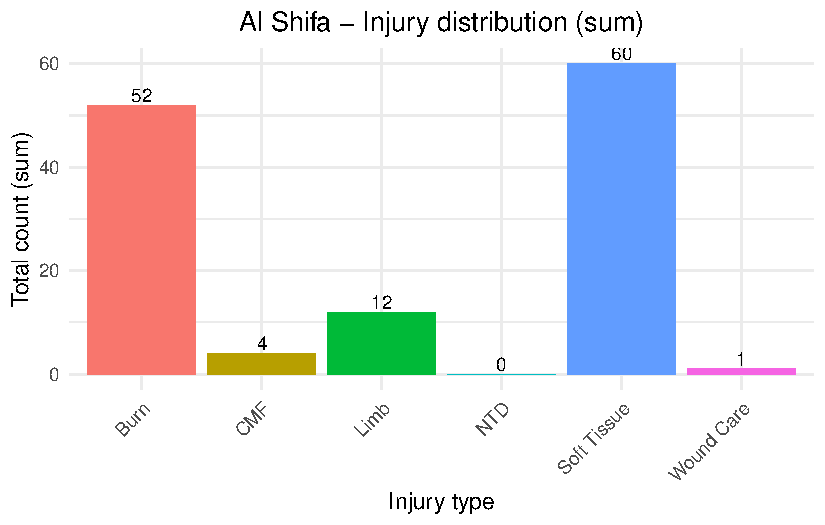
\includegraphics[keepaspectratio]{EDA_files/figure-pdf/injury-distributions-by-hospital-1.pdf}}

\pandocbounded{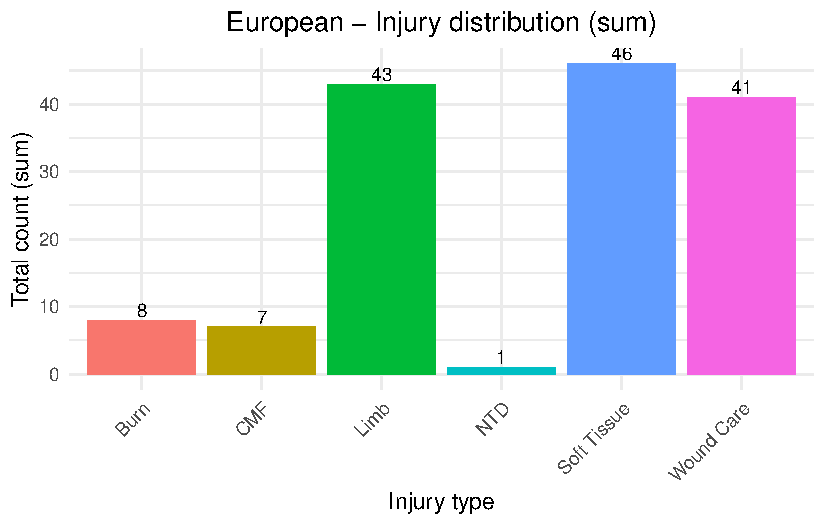
\includegraphics[keepaspectratio]{EDA_files/figure-pdf/injury-distributions-by-hospital-2.pdf}}

\pandocbounded{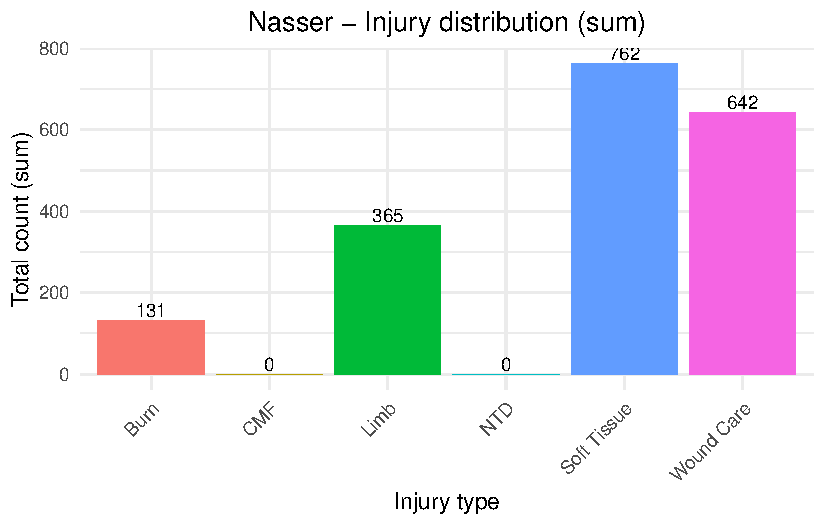
\includegraphics[keepaspectratio]{EDA_files/figure-pdf/injury-distributions-by-hospital-3.pdf}}

\begin{Shaded}
\begin{Highlighting}[]
\CommentTok{\# {-}{-}{-} 6) Combined faceted bar plot (3 panels) for comparison {-}{-}{-}}
\NormalTok{p\_combined }\OtherTok{\textless{}{-}}\NormalTok{ ggplot2}\SpecialCharTok{::}\FunctionTok{ggplot}\NormalTok{(summary\_combined, ggplot2}\SpecialCharTok{::}\FunctionTok{aes}\NormalTok{(}\AttributeTok{x =}\NormalTok{ injury\_label, }\AttributeTok{y =}\NormalTok{ count, }\AttributeTok{fill =}\NormalTok{ injury\_label)) }\SpecialCharTok{+}
\NormalTok{  ggplot2}\SpecialCharTok{::}\FunctionTok{geom\_col}\NormalTok{(}\AttributeTok{show.legend =} \ConstantTok{FALSE}\NormalTok{) }\SpecialCharTok{+}
\NormalTok{  ggplot2}\SpecialCharTok{::}\FunctionTok{geom\_text}\NormalTok{(ggplot2}\SpecialCharTok{::}\FunctionTok{aes}\NormalTok{(}\AttributeTok{label =}\NormalTok{ count), }\AttributeTok{vjust =} \SpecialCharTok{{-}}\FloatTok{0.25}\NormalTok{, }\AttributeTok{size =} \DecValTok{3}\NormalTok{) }\SpecialCharTok{+}
\NormalTok{  ggplot2}\SpecialCharTok{::}\FunctionTok{facet\_wrap}\NormalTok{(}\SpecialCharTok{\textasciitilde{}}\NormalTok{ hospital, }\AttributeTok{scales =} \StringTok{"free\_y"}\NormalTok{) }\SpecialCharTok{+}
\NormalTok{  ggplot2}\SpecialCharTok{::}\FunctionTok{labs}\NormalTok{(}\AttributeTok{title =} \StringTok{"Injury distribution by hospital (sum of counts per injury type)"}\NormalTok{,}
                \AttributeTok{x =} \StringTok{"Injury type"}\NormalTok{, }\AttributeTok{y =} \StringTok{"Total count (sum)"}\NormalTok{) }\SpecialCharTok{+}
\NormalTok{  ggplot2}\SpecialCharTok{::}\FunctionTok{theme\_minimal}\NormalTok{() }\SpecialCharTok{+}
\NormalTok{  ggplot2}\SpecialCharTok{::}\FunctionTok{theme}\NormalTok{(}\AttributeTok{axis.text.x =}\NormalTok{ ggplot2}\SpecialCharTok{::}\FunctionTok{element\_text}\NormalTok{(}\AttributeTok{angle =} \DecValTok{45}\NormalTok{, }\AttributeTok{hjust =} \DecValTok{1}\NormalTok{),}
                 \AttributeTok{plot.title =}\NormalTok{ ggplot2}\SpecialCharTok{::}\FunctionTok{element\_text}\NormalTok{(}\AttributeTok{hjust =} \FloatTok{0.5}\NormalTok{))}

\FunctionTok{print}\NormalTok{(p\_combined)}
\end{Highlighting}
\end{Shaded}

\pandocbounded{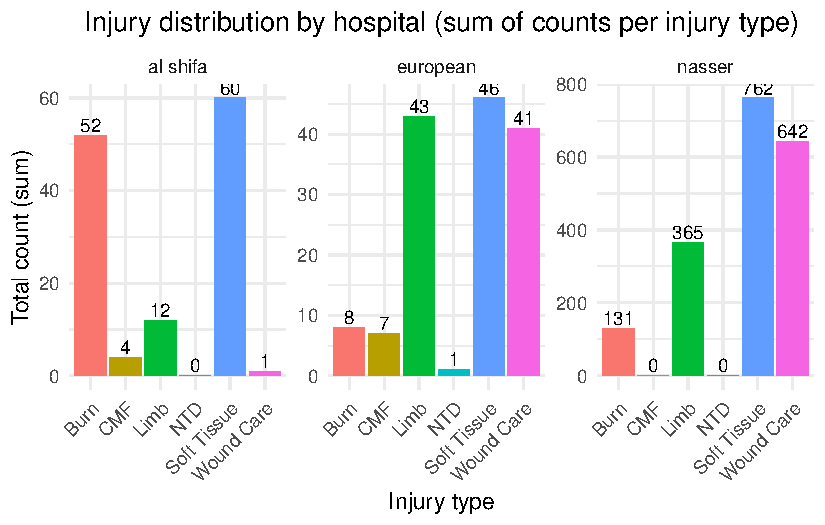
\includegraphics[keepaspectratio]{EDA_files/figure-pdf/injury-distributions-by-hospital-4.pdf}}

\begin{Shaded}
\begin{Highlighting}[]
\CommentTok{\# {-}{-}{-} End {-}{-}{-}}
\CommentTok{\# Notes:}
\CommentTok{\# {-} If any hospital returned "no rows found" or had zero sums, check your hospital column and hospital names in the spreadsheet.}
\CommentTok{\# {-} If you\textquotesingle{}d like the hospital display names to be exactly "Al Shifa Medical Hospital", "European Hospital", "Nasser Hospital", replace the \textasciigrave{}hospital\_targets\textasciigrave{} vector with the desired display strings and adjust the matching patterns (or provide exact strings).}
\CommentTok{\# {-} Want the counts normalized (percent of hospital) instead of raw sums? I can add that.}
\end{Highlighting}
\end{Shaded}





\end{document}
